%!TEX root = ../masters_thesis.tex

\chapter{Development} % (fold)
\label{cha:development}

The aim of this thesis is to create a Historical Geographic Information System to visualize and edit the evolution of countries in time and space. This is a complicated task, because both the reality and the human that should be able to use the system are complex. The task is to create an interface that a human can easily understand and use. For complex applications in which the interface matters, the methodologies of \emph{Human Centered Design} are promising to achieve a good solution.

The development process is iterative divided in several phases. In each phase, the fidelty towards the final solution is increased. A phase starts with an initial set of requirements about the problem. In multiple iterations, an interface is developed that solves the problem. Each iteration has four steps: The requirements for the system are analyzed in the \emph{planning} step. Afterwards, they translated into an abstract \emph{design} which is realized in a specific \emph{implementation} of the interface. Finally, this interface is tested with humans to find out how well it works. Based on the results of this \emph{testing} step, the requirements are updated and the next iteration starts. This is repeated until a version of the interface is created that sufficiently solves the problem. Then the fidelity is increased, starting the next development phase.

The five phases in this thesis were:
\begin{compactenum}
  \item \textbf{Idea}: The initial idea how to edit and visualize the history of countries.
  \item \textbf{Paper Prototype}: The concept of the interface realized and tested on paper.
  \item \textbf{Mockup Prototype}: The concrete workflow developed in a slide-based presentation.
  \item \textbf{Web-Based Prototype}: The final version developed in a Web application.
  \item \textbf{Extensions}: Design approaches how to fit the uncertain nature of history.
\end{compactenum}

\begin{figure}[H]
  \centering
  \includegraphics[width=0.8\textwidth]{graphics/development/hcd}
  \caption{Human Centered Design process with five project phases}
  \label{fig:hcd}
\end{figure}

There are several models involved in the development of the software, each of them has to be developed or analyzed separately. The \emph{data model} is an abstraction and simplification of the real world. The \emph{Hivent Model} created in this thesis is explained in the first section \ref{sec:hivent_model} of this chapter. In iteractive computer systems, the \emph{mental model} is the representation in the mind of the human about how the interface he or she is interacting with should work. On the other hand, the \emph{conceptual model} describes the way the interface actually works. The goal of Human Centered Design is to match the conceptual model to the mental model. Section \ref{sec:histoglobe_interface} outlines the gradual interface design process to reach this goal. In the application, the implemented \emph{database model} has to match the abstract data model. The task for the \emph{computational model} is to translate between the database model and the conceptual model. The working of the HistoGlobe application, including the computational model, is introduced in the last section \ref{sec:histoglobe_application} of this chapter.

\begin{figure}[H]
  \vspace{1em}
  \centering
  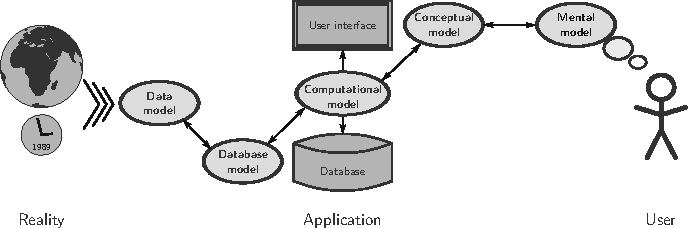
\includegraphics[width=0.8\textwidth]{graphics/development/models}
  \caption{Relevant models for the system}
  \label{fig:models}
\end{figure}

% ==============================================================================
%!TEX root = ../masters_thesis.tex

\section{Hivent Model} % (fold)
\label{sec:hivent_model}

This section introduces the data model that represents countries and their evolution in time and space. In section \ref{sec:spatio_temporal_data_models}, different spatio-temporal data models were introduced to solve this problem. The \emph{Snapshot Model} is unsuitable for the problem space. \emph{Simple Time-Stamping} is helpful to link countries to their history, but it does not explicitly model historical changes, which is desireable. For that purpose, the idea of the \emph{Event-Based Spatio-Temporal Data Model} was developed, but since it only works for raster data, it is also not suitable for this thesis. This problem is solved in the \emph{History Graph Model}. Additionally, the introduced temporal changes allow to represent historical changes and their influences on geographic entities directly in the model. Finally, the \emph{Three-Domain Model} introduces a helpful concept to separate the spatial, temporal and thematic dimension of a spatio-temporal entity.

The \emph{Hivent Model} is constructed from components of some of these models: An Event-Based Spatio-Temporal Data Model supporting vector data. It is organized according to the Three-Domain Model, uses Simple Time-Stamping to define the lifetime of a spatial entity, and to visualize it on a History Graph. In the first section of this section, the main elements of the Hivent model are introduced. Afterwards, the preconditions are defined. Finally, the Historical Geographic Operations that describe changes of countries in time and space are explained.

% ------------------------------------------------------------------------------
\subsection{Elements} % (fold)
\label{sub:elements}

The main elements of the the model are \emph{Hivent}s, representing an historically significant happening and \emph{Area}s, an abstract entity on a map with a name and a territory. An \emph{Historical Change} is part of one Hivent and manipulates the history of one or more Areas.

% - - - - - - - - - - - - - - - - - - - - - - - - - - - - - - - - - - - - - - -
\vspace{-1em}
\paragraph{Hivents} % (fold)
\label{par:hivent}

are the main organizing elements of the data model. The word is an acronym for \emph{\textbf{Hi}}storical e\emph{\textbf{vent}}. It represents a significant happening in history, e.g. a treaty, bill or declaration. The focus in this work is on events that influence the geopolitical situation on Earth. An Hivent happens at one particular point in time and space and introduces historical changes to countries.

% paragraph hivent (end)

% - - - - - - - - - - - - - - - - - - - - - - - - - - - - - - - - - - - - - - -
\vspace{-1em}
\paragraph{Areas} % (fold)
\label{par:area}

represent one identical current or historical country with a \emph{name} and a \emph{territory} on the map. The name of the Area consists of a common \emph{short name}, e.g. ``Germany'' and a \emph{formal name}, e.g. ``Federal Republic of Germany''. The \emph{territory} of the Area is described by a polypolygon, a set of weakly simple polygons to support enclaves and exclaves. The polylines of the polygons consist of an ordered set of points that represent the country border. The borders of a country are either \emph{interior}, i.e. bordering another country, or a \emph{coastline}, bordering a body of water.

% paragraph area (end)

% ------------------------------------------------------------------------------
\vspace{-1em}
\paragraph{Historical Changes} % (fold)
\label{par:historical_changes}

influence the development of an Area over time. Throughout the lifetime of an Area, it is created at some point $t_s$, then its territory and short name can change multiple times $t_i: t_s < t_i$ and at some point $t_e: t_s < t_i < t_e$ it ceases. Since all changes in this model are sudden, there are only two possible states an Area can be in: It is \emph{active}, if at the current time point it is historically existing and it is \emph{inactive} if it does not. Each area is uniquely identified by its formal name. That means, the short name can change, but as soon as the formal name of an area changes (e.g. ``German Empire'' to ``Federal Republic of Germany''), it is considered a ``new'' Area.

Each Historical Change belongs to exactly one Hivent, inheriting its time point at which the change happens.  The change is described by a Historical Geographic Operation introduced in section \ref{sub:historical_geographic_operations}.

\begin{figure}[H]
  \vspace{1em}
  \centering
  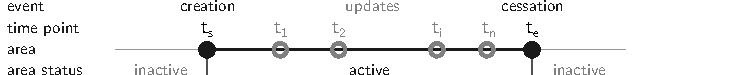
\includegraphics[width=0.9\textwidth]{graphics/development/area_states}
  \caption{Three event types that change Areas, resulting in two different area states}
  \label{fig:area_states}
\end{figure}


% paragraph historical_changes (end)

% subsection section area (end)

% ------------------------------------------------------------------------------
\subsection{Preconditions} % (fold)
\label{sub:preconditions}

\begin{quoteit}
In the beginning God created the heavens and the Earth \\
Now the Earth was formless and empty [...] \\
And God said, “Let there be light” --- and there was light.
\end{quoteit}
\hfill -- Genesis 1:1, The First Book of Moses, Old Testament

There are five axoims and two assumptions that are the basis of the spatio-temporal system developed in this thesis. The theoretical foundation is the model of the Earth, its curved surface that can be projected on a two-dimensional map using a map projection, as introduced in sections \ref{sub:model_of_geographical_space} and \ref{sub:presentation_of_geographic_space}.

\vspace{-1.0em}
\newtheorem{invariant_surface}[assicounter]{Axiom}
\begin{invariant_surface}
\label{axm:invariant_surface}
  The Earth's surface has an invariant area size, i.e. it does not change over time.
\end{invariant_surface}

\vspace{-2.5em}
\newtheorem{area_on_surface}[assicounter]{Axiom}
\begin{area_on_surface}
\label{axm:area_on_surface}
  Each Area in the spatio-temporal system is located directly on the surface of the Earth.
\end{area_on_surface}

These axiom sets the spatial foundation of the system: a constant dimension of the map and Areas covering the map. The basis of the temporal part of the system is content of the next three axioms:

\vspace{-1.0em}
\newtheorem{initial_configuration}[assicounter]{Axiom}
\begin{initial_configuration}
\label{axm:initial_configuration}
  The spatio-temporal system has an initial state at time point $t_0$. At this initial state, there exists exactly one Area, denoted by $\Omega$ and referred to as the \emph{universe} Area. It has no name and its territory covers the whole surface of the Earth.
\end{initial_configuration}

\vspace{-2.5em}
\newtheorem{historical_change}[assicounter]{Axiom}
\begin{historical_change}
\label{axm:historical_change}
  At each time point $t_i \geq t_0$ an Historical Change can be introduced.
\end{historical_change}

\vspace{-2.5em}
\newtheorem{unique_coverage}[assicounter]{Axiom}
\begin{unique_coverage}
\label{axm:unique_coverage}
  At each time point $t_i \geq t_0$ each point on the surface of the Earth is covered by exactly one territory of exactly one Area.
\end{unique_coverage}

As it has been defined in section \ref{par:historical_changes}, an Historical Change can create, manipulate and cease Areas on the Earth's surface. According to axoim \ref{axm:unique_coverage}, each change introduced in the system must maintain the spatial integrity on the map: When an Area with a territory is created on the map, the Area claiming this territory before has to cease this territory. Formally, it can be said that each change consists of a set of old Areas $A$ that are manipulated, a set of new Areas $B$ that are created in the change, and an operation $\rightarrow_C$ describing the change. Each Area $A_i \in A$ and $B_i \in B$ has a territory $A_i^T$  respectively $B_i^T$. For each change introduced in the system, the territories of the old Areas must have the same size than the territories of the new Areas to maintain the spatial integrity of axiom \ref{axm:unique_coverage}:
\begin{align}
  \bigcup\limits_{i=1}^n A_i^T ~\textbf{=}~ \bigcup\limits_{i=1}^n B_i^T
\end{align}

The first Historical Changes introduced in the system at time point $t_0$ are the creation of all bodies of water, including the oceans and lakes, denoted as $W$. Each Area $W_i \in W$ is created with their name and territory cut out of $\Omega$. The result is that at $t_0$, the map is divided into water ($W$) and land ($\Omega$). Land can at any point in time be either \emph{claimed}, i.e. it is currently occupied by the territory of exactly one active Area, or on a contrary be \emph{unclaimed}, i.e. belonging to $\Omega$. It is a subtractive data model, because each new Areas territory is cut out of $\Omega$.

\begin{figure}[H]
  \centering
  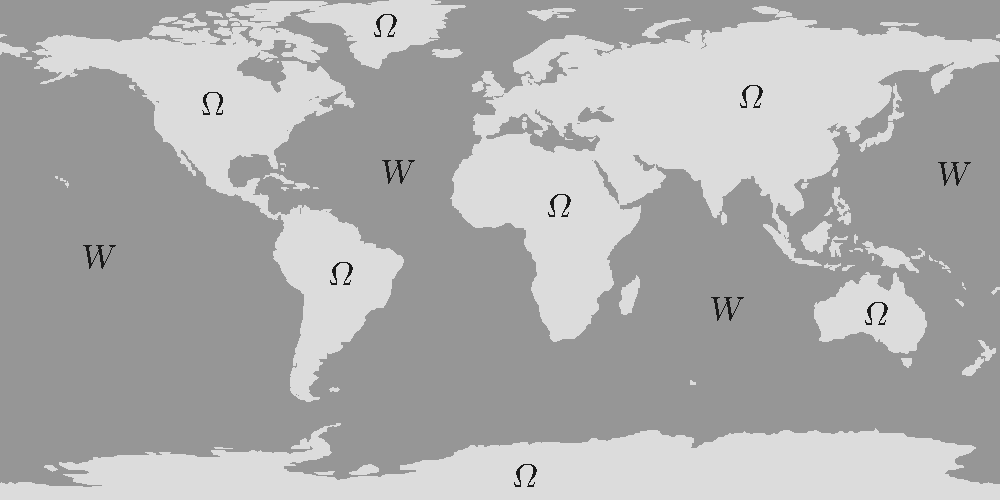
\includegraphics[width=0.5\textwidth]{graphics/development/init_map}
  \caption{The initial state of the world map at time point $t_0$}
  \label{fig:init_map}
\end{figure}

In the real world, the name of a country changes according to sudden events, e.g. a declaration or a governmental bill. The territory can change either because of a geographical processes, e.g. the sea level rise influencing the change of the coastline, or according to a historical event, e.g. a treaty. The Hivent model is based on two assumptions that simplify the model and keep the problem space clear:

\vspace{-1.0em}
\newtheorem{coastline_territory}[assicounter]{Assumption}
\begin{coastline_territory}
\label{axm:coastline_territory}
  The territory of a country stops at the coastline.
\end{coastline_territory}

\vspace{-1.5em}
\newtheorem{constant_coastlines}[assicounter]{Assumption}
\begin{constant_coastlines}
\label{axm:constant_coastlines}
  The spatial configuration of the Earth's surface, i.e. land, water and the coastlines, has not changed over time.
\end{constant_coastlines}

Both assumptions are obviously wrong: In line with \cite{UNSeaBorders}, the territory of a country extends in a range of 3 to 12 miles (5 to 20 kilometers) into international waters. They are constantly changing and so does the distribution of land and water on Earth. However, the assumptions allow the Hivent Model to focus only on discrete historical changes and not on long-term processes. In this data model, the temporal behavior of an Area can therefore be described as a \emph{static object that changes according to sudden events}.

% base: Newtons concept of absolute space?
% TODO: topological rule?
% each border has exactly two neighboring Areas
% each Area has at least one neighboring Area

% subsection preconditions (end)

% ------------------------------------------------------------------------------
\subsection{Historical Geographic Operations} % (fold)
\label{sub:historical_geographic_operations}

Respecting the preconditions, there are several different types of changes that can occur to a set of Areas. All possible changes can be expressed with only five spatio-temporal operations that are called \emph{Historical Geographic Operations} (HG Operations). The first four change the identity of a set of Areas and therefore establish historical predecessor-successor-relationships. They are always symmetric, i.e. if one old Area is replaced by one new Area, the old Area is the historical predecessor of the new Area and vice versa the new Area is the successor of the old Area.

\begin{description}
  \item[UNI -- Unification]
  A set of old Areas unifies to one new Area. The old Areas cease, becoming the historical predecessors of the new Area. This new Area receives a new name and its territory is the union of the territories of the old Areas. \\[0.25em]
  \begin{footnotesize}
    In 1922, the Russian SFSR, the Transcaucasian SFSR, the Ukrainian SSR and the Byelorussian SSR unified and formed the Union of Soviet Socialist Republics (USSR).
  \end{footnotesize}
  \item[INC -- Incorporation]
  One or more old Areas are incorporated into another Area that stays active. Its territory is enlarged by the union of the territories of the old Areas. The old Areas are historical predecessors of the new Area. \\[0.25em]
  \begin{footnotesize}
    In 1990, the territory of the German Democratic Republic (East Germany) became part of the Federal Republic of Germany (West Germany). Although this event is known as the \emph{German Reunification}, it is historically an incorporation of East Germany into West Germany \cite{incorporationEastWestGermany}.
  \end{footnotesize}
  \item[SEP -- Separation]
  As the inverse of unification, one old Area is preceded by multiple new Areas. Each new Area gets a new name, receives a part of the territory of the old Area, and the old Area as its only historical predecessor. \\[0.25em]
  \begin{footnotesize}
    In 1993, the Czech and Slovak Federal Republic, commonly known as Czechoslovakia, dissolved into present-day Czech Republic and Solvak Republic, creating two new countries out of one old.
  \end{footnotesize}
  \item[SEC -- Secession]
  As the inverse of incorporation, one or more new areas are ceded from a previously exising area that stays active. Each new Area gets a new name, receives the previously existing Area as the only historical predecessor and a part of its territory. \\[0.25em]
  \begin{footnotesize}
    In 2008, the Republic of Kosovo declared independence from Serbia and has since then partially received international recognition. Unlike in the case of separation, Serbia stays as country, keeping its name, but ceding a part of its territory to Kosovo.
  \end{footnotesize}
  \item[NCH -- Name Change]
  An Area changes its short name but preserves its identity. \\[0.25em]
  \begin{footnotesize}
    A recent change happened on 5. May 2016: The cabinet of Czech Republic approved that the country will now offically be called ``Czechia''. However, the formal name stays ``Czech Republic'', which preserves its identity.
  \end{footnotesize}
\end{description}

HG Operations can be combined when they happen at the same time, e.g. if one Area incorporates another Area and thereby changes its short name, this is a combination of \texttt{INC + NCH}. When West Germany incorporated East Germany in 1900, it was from that moment on just called Germany.

% - - - - - - - - - - - - - - - - - - - - - - - - - - - - - - - - - - - - - - -
\begin{table}[H]
\begin{center}
\begin{tabular}{m{0.75cm} m{2.5cm} m{2.5cm} cx{2.5cm}}
  \toprule
  & operation
  & \multicolumn{1}{c}{visualization}
  & \multicolumn{1}{c}{\pbox{2.5cm}{historical\\relationship\protect\footnotemark}} \\

  \midrule
  \texttt{UNI} & Unification & \raisebox{-0.25\height}
  {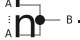
\includegraphics{graphics/development/hg_operations/UNI}} &
  $ A_i \leftrightarrow_H B_1 $ \\

  \midrule
  \texttt{INC} & Incorporation & \raisebox{-0.25\height}
  {
\includegraphics{graphics/development/hg_operations/INC}} &
  $ A_i \leftrightarrow_H A_0 $ \\

  \midrule
  \texttt{SEP} & Separation & \raisebox{-0.25\height}
  {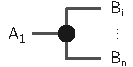
\includegraphics{graphics/development/hg_operations/SEP}} &
  $ A_1 \leftrightarrow_H B_i $ \\

  \midrule
  \texttt{SEC} & Secession & \raisebox{-0.25\height}
  {
\includegraphics{graphics/development/hg_operations/SEC}} &
  $ A_0 \leftrightarrow_H B_i $ \\

  \midrule
  \texttt{NCH} & Name Change & \raisebox{-0.25\height}
  {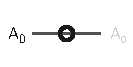
\includegraphics{graphics/development/hg_operations/NCH}} &
  $ \emptyset $ \\

  \bottomrule
\end{tabular}
\caption{The five HG Operations}
\label{tab:historical_geographic_operations}
\end{center}
\end{table}

\footnotetext{$A_i \leftrightarrow_H B_i$ denotes: $\forall i \in [1..n]:$ $A_i$ is historical predecessor of $B_i$ and $B_i$ is successor of $A_i$}

% subsection historical_geographic_operations (end)

% ------------------------------------------------------------------------------
\subsection{Edit Operations} % (fold)
\label{sub:edit_operations}

The Historical Geographic Operations are a valuable set of tools to describe all kinds of changes in the evolution of countries in time and space. They are really well understood from the system point of view and are therefore the basis for the Hivent Model. However, the purpose of the HGIS developed in this thesis is to provide an interface for the user to introduce historical changes to countries on the map.

Throughout the development process, interviews with historians and other researchers in humanities at University of Virginia were conducted, to understand their mental model about historical changes of countries. In the interviews it turned out that the HG Operations are not suitable to be used for human edit purposes, because of their low-level nature. One example is that the operations do not provide a straightforward way to create a new country on previously unclaimed land. The same is true for changing the formal name of an Area.

Therefore, this thesis introduces a second set of high-level operations to introduce changes to countries on the map: the \emph{Edit Operations} in table \ref{tab:edit_operations} have proven to be understandable in several user studies.

\begin{table}[H]
\begin{center}
\begin{tabular}{m{0.75cm} m{0.8cm} m{2.4cm} m{9.1cm}}
  \raisebox{-0.35\height}
  {
\includegraphics[width=0.72cm]{graphics/development/edit_operations/CRE}} &
  \texttt{CRE} & Create &
  a new Area with a new name and territory on the map. \\

  \raisebox{-0.35\height}
  {
\includegraphics[width=0.72cm]{graphics/development/edit_operations/MRG}} &
  \texttt{MRG} & Merge &
  two or more Areas to a new Area. The name has to be set manually, the territory is automatically unified. \\

  \raisebox{-0.35\height}
  {
\includegraphics[width=0.72cm]{graphics/development/edit_operations/DIS}} &
  \texttt{DIS} & Dissolve &
  one Area into two or more new Areas, manually setting their new territory and name. \\

  \raisebox{-0.35\height}
  {
\includegraphics[width=0.72cm]{graphics/development/edit_operations/CHB}} &
  \texttt{CHB} & Change Borders &
  between two neighboring Areas by defining the territory that changes sides. \\

  \raisebox{-0.35\height}
  {
\includegraphics[width=0.72cm]{graphics/development/edit_operations/REN}} &
  \texttt{REN} & Rename &
  an Area and set a new formal name, short name or both. \\

  \vspace{0.35em}
  \raisebox{-0.35\height}
  {
\includegraphics[width=0.72cm]{graphics/development/edit_operations/CES}} &
  \texttt{CES} & Cease &
  an Area by deleting it from the map, leaving unclaimed land. \\

\end{tabular}
\caption{The six Edit Operations}
\label{tab:edit_operations}
\end{center}
\end{table}


% subsection edit_operations (end)

% section hivent_model (end)
%!TEX root = ../masters_thesis.tex

\section{HistoGlobe Interface} % (fold)
\label{sec:histoglobe_interface}

The Hivent Model presented in the previous section is the data model for HistoGlobe, the application in which the work of this thesis is implemented in. Developing the system bottom-up from the data model to the interface might lead to a system that is not well usable. Human Centered Design promotes a top-down process from the user via the interface into the core of the application. Figure \ref{fig:hcd} shows the five phases that lead from the identification of the mental model of the user all the way to the final interface and possible extensions to it that were not yet implemented. This section illustrates the iterative design process for this thesis. The two main use cases for HistoGlobe that are focused in this thesis are:

\begin{compactenum}
  \item \textbf{Understanding} the history of countries.
  \item \textbf{Editing} the spatio-temporal evolution of countries with historical changes.
\end{compactenum}

For both use cases a visualization and interaction was designed. The interviews with humanity researchers confirmed that the combination of a map and a timeline are a very appropriate and intuitive way to interactively visualize the history of countries. Thefore, the main concept of HistoGlobe introduced in section \ref{sec:histoglobe} does not need to be changed.

However, two necessary extension modules have emerged: The \emph{HistoGraph} visualizes the history of countries aspatially on a graph. Its main idea is introduced in section \ref{sub:histograph}. Next to the normal exploration mode with map, timeline and HistoGraph, the concept of the \emph{Edit Mode} based on the Edit Operations to manipulate historical changes is proposed in section \ref{sub:editmode}. The gradual process from the inital idea to the final user interface implemented in HistoGlobe is illustrated in the last section \ref{sub:design_iterations}.

% ------------------------------------------------------------------------------
\subsection{HistoGraph} % (fold)
\label{sub:histograph}

Based on the idea of the History Graph Model (section \ref{fig:history_graph_model}), the linguistically and conceptually related \emph{HistoGraph} visualizes the history of countries on a graph. The edges of the graph represent an Area, the nodes an Hivent that changes the Areas evolution. The graph focuses on the historical, rather than the spatial aspect of countries: the predecessor-successor-relationships between Areas to trace the evolution throughout time. This is easily possible because of the usage of Simple Time-Stamping, one feature of the Hivent Model.

The two-dimensional HistoGraph has an horizontal orientation. It expands the timeline: the x-axis of the graph refers to one time point. The y-axis has no spatial or temporal relation, its dimension changes depending on how much space the visualization needs. The graph uses the visualization approach of the five HG Operations (table \ref{tab:historical_geographic_operations}), including the following symbols (table \ref{tab:histograph_symbols}):

\begin{table}[H]
\begin{center}
\begin{tabular}{c l l}

  \raisebox{3.5\height}
  {
\includegraphics{graphics/development/histograph/line}}
  & Area
  & \\

  \raisebox{-0.2\height}
  {
\includegraphics{graphics/development/histograph/circle_filled}}
  & Identity-changing HG Operation
  & \texttt{UNI}, \texttt{INC}, \texttt{SEP}, \texttt{SEC} \\

  \raisebox{-0.2\height}
  {
\includegraphics{graphics/development/histograph/circle_unfilled}}
  & Property-changing HG Operation
  & \texttt{NCH} \\

  \raisebox{-0.2\height}
  {
\includegraphics{graphics/development/histograph/circle_combo}}
  & A combination of both
  & e.g. \texttt{INC + NCH} \\

\end{tabular}
\caption{symbols used in the HistoGraph}
\label{tab:histograph_symbols}
\end{center}
\end{table}

Each uninterrupted horizontal line refers to exactly one identical Area. New Areas resulting from an identity-changing HG Operation, emerge from an operation with a vertical line, indicating a sudden change with zero duration. From this line, the new Areas branch out right-angled. A horizontal line going straight through a circle indicates that the identity of the Area was preserved in the operation.

The HistoGraph is always created starting from one particular reference Area. It visualizes historically related Areas in one direction. That means, in historically backward direction, it recursively plots the predecessors on the graph, but not the predecessors successors. In the opposite historically forward direction, recursively the successors of the reference Area are plotted, but not their predecessors.

\begin{figure}[H]
  \vspace{1em}
  \centering
  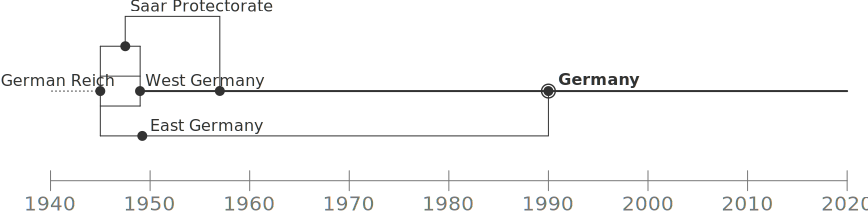
\includegraphics[width=0.8\textwidth]{graphics/development/histograph/example_germany}
  \caption{The concept of the HistoGraph at the example of the history of Germany since 1945}
  \label{fig:example_germany}
\end{figure}

The behavior of the HistoGraph is shown in figure \ref{fig:example_germany} at the example of present-day Germany and its state history since the end of World War II. This history was driven by six historical events, which provide examples for all five HG Operations (table \ref{tab:german_history_since_1945}). The graph first plots Germany. Since it does not have any successors, the plot goes only one way, historically backwards: East Germany and the Saar Protectorate were incorporated into Germany, so they are plotted. All emerged from the four post-war occupation zones, which are also plotted. All of the four occupation zones themselves originated from the German Reich. However, the German Reich dissolved into many more Areas, e.g. the Memel territory. They are not included in the graph, because they are not predecessors of any Area that is a recursive predecessor of present-day Germany.

\begin{table}[H]
\begin{center}
\begin{tabular}{l p{8.5cm} l}
  \toprule
  Hivent date & Hivent description & HG Operations \\
  \midrule

    05.06.1945
  & \footnotesize{In the Berlin Declaration the total dissolution of the Third German Reich is confirmed. It separated into several different parts, returning the territories annexed by the German Reich in World War II to their original countries. The rest is controlled by the Allied Control Council in four occupation zones: the British, French, American and Soviet occupation zone.}
  & \texttt{SEP} \\

    16.02.1946
  & \footnotesize{The Saar Protectorate is entangled from the French Zone of Occupation Germany, creating an own country.}
  & \texttt{SEC} \\

    28.05.1949
  & \footnotesize{The Federal Republic of Germany (West Germany) is created from the British, American and French Zone of Occupation.}
  & \texttt{UNI} \\

    07.10.1949
  & \footnotesize{The German Democratic Republic (East Germany) is created from the Soviet Zone of Occupation}
  & \texttt{UNI} \\

    01.01.1957
  & \footnotesize{The Saar Treaty (``Little Reunification'') joins the Saar Protectorate as the Bundesland Saarland in West Germany.}
  & \texttt{INC} \\

    03.10.1990
  & \footnotesize{In the German Reunification, East Germany joins West Germany. The Federal Republic of Germany is now just called ``Germany''.}
  & \texttt{INC + NCH} \\

  \bottomrule
\end{tabular}
\caption{Historical events in German state history since 1945}
\label{tab:german_history_since_1945}
\end{center}
\end{table}

The example hosts a special case: in October 1949, East Germany was created from the Soviet Zone of occupation. Both Areas have the same territory, but a different short and formal name. A \texttt{NCH} can not be performed, because the identity is not preserved: The German Democratic Republic is a new Area. However, the change can be described by a \texttt{UNI} of only one Area (Soviet Zone), creating a new Area (East Germany) and establishing a historical relationship between both.

Many problems of the graph visualization are apparent in this example: If many operations happened in a short period of time (in this case between 1945 and 1949), dots might overlap.
The name ``West Germany'' collides with the vertical line indicating the incorporation of the Saar Protectorate, which should also be avoided.
Additionally, the names of the Areas of the four post-war occupation zones can not be shown in the Graph, because there is no space for them.
One more important aspect can be seen in the creation of West Germany in 1949: A \texttt{UNI} operation unifies three old Areas to one new Area. This could be visualized symmetrically with a straight line from the midmost incoming Area line into the Hivent circle to the outgoing Area line of the new Area. This would give the impression that this midmost Area has the same identity than the newly created Area, which is not the case. Therefore, the Hivent circle for \texttt{UNI} and \texttt{SEP} operations with an add number of old respectively new Areas must be displaced off the center to emphasize that the identity has changed.
All these issues are not in the scope of this thesis and subject to future work in the field of Information Visualization.

% subsection histograph (end)

% ------------------------------------------------------------------------------
\subsection{Edit Mode} % (fold)
\label{sub:edit_mode}

The user interface of HistoGlobe has two modi: The exploration mode to view the evolution of countries on a map with a timeline and a HistoGraph and the \emph{Edit Mode} proposed in this section. In the Human Centered Design process of this thesis, an interface was found that allows to intuitively edit historical changes directly in HistoGlobe, without the need to write data into database tables or standardised forms. There two main use cases in the Edit Mode:

\begin{compactenum}
  \item \textbf{Introducing an historical change} to Areas on the map.
  \item \textbf{Correcting} the name or the territory of an Area on the map.
\end{compactenum}

Looking at the data model, both use cases lead to the same result: If the information at one point in history $t_1$ is wrong, e.g. the name of country $X$ should actually be $Y$, this means that the historical change that created name $X$ at time point $t_0$ is erroneous and has be corrected. Especially if $t_0$ is far away in the past, the studies have shown that altering an historical change to correct an information on a map now is not very intuitive. Therefore, the Edit Mode is designed to serve both use cases.

The conceptual model promotes the six Edit Operations (section \ref{sub:edit_operations}) that humans can understand, the data model is based on five HG Operations (section \ref{tab:historical_geographic_operations}) that can model all evolutionary changes to countries in time and space. Therefore the task for the computational model of HistoGlobe is to translate between both operation sets.


% - - - - - - - - - - - - - - - - - - - - - - - - - - - - - - - - - - - - - - -
\paragraph{Workflow} % (fold)
\label{par:workflow}

This happens in a workflow with four steps. They are based on the idea, that an historical change, described by an Edit Operation, transformes a set of old areas to a set of new areas.

\begin{enumerate}
  \item \texttt{SELECT\_OLD\_AREAS}: The user selects the old Areas that will be changed in the Edit Operation.
  \item \texttt{CREATE\_NEW\_TERRITORIES}: For each new Area resulting from the Edit Operation, the user creates a polypolygon describing the territory of the Area.
  \item \texttt{CREATE\_NEW\_NAMES}: Afterwards the user writes the name of each new Area directly on the map. This finalizes the set of new Areas for the historical change.
  \item \texttt{ADD\_CHANGE}: Finally, the historical change has to be added to an Hivent that introduces it and inherits the time point to it. The user either selects an existing Hivent or creates a new one. All the information necessary for the spatio-temporal Hivent Model are completed.
\end{enumerate}

For each Edit Operation, the requirements for the steps are different. Not all operations need all steps and some data is processed automatically. Table \ref{tab:editoperations_in_worklow} presents an overview about the behaviour of each operation in the first three steps. The last step is the same for each operation: Adding the historical change to an Hivent.

\begin{table}[H]
\begin{center}
\begin{tabular}{m{0.9cm} m{4.0cm} m{4.4cm} m{3.8cm}}
  \toprule

  &
  \texttt{SELECT\_OLD\_AREAS} &
  \texttt{CREATE\_NEW\_TERRITORIES} &
  \texttt{CREATE\_NEW\_NAMES} \\

  \midrule
  \texttt{CRE} &
  -- &
  \pbox{4.4cm}{create a territory of the new country\\
  \footnotesize{on unclaimed land and/or overlapping existing countries}} &
  create a name of the new country \\

  \midrule
  \texttt{MRG} &
  select the countries to be merged &
  \pbox{4.4cm}{--\\
  \footnotesize{automatic unification of territories of selected countries}} &
  create a name of the merged country
  \\

  \midrule
  \texttt{DIS} &
  select a country to be \mbox{dissolved} &
  create a territory for each new country &
  create a name for each new country \\

  \midrule
  \texttt{CHB} &
  select two neighboring countries to change their border &
  \pbox{4.4cm}{create the new border between both countries \\
  \footnotesize{the territory for both countries will be created automatically}}  &
  -- \\

  \midrule
  \texttt{REN} &
  select a country to change its name &
  -- &
  create a new name of the country \\

  \midrule
  \texttt{CES} &
  select a country to cease it &
  -- &
  -- \\

  \bottomrule
\end{tabular}
\caption{The requirements of each step for the Edit Operations}
\label{tab:editoperations_in_worklow}
\end{center}
\end{table}

% paragraph workflow (end)

% subsection edit_mode (end)

% ------------------------------------------------------------------------------
\subsection{Design Iterations} % (fold)
\label{sub:design_iterations}

The previous two sections introduced the concept of the HistoGraph and the Edit Mode. This section presents the gradual Human Centered Design process integrating both concepts in the existing HistoGlobe user interface. In each step, interviews with students and employees of the Scholar's Lab of University of Virginia were conducted to find out what works well and to identify current problems and design flaws.

% - - - - - - - - - - - - - - - - - - - - - - - - - - - - - - - - - - - - - - -
\paragraph{Initial interviews} % (fold)
\label{par:initial_interviews}

The first step was an interview with four researchers asking about their comments to the idea of HistoGlobe, potential use cases and the concept of the Edit Mode. The result was that the idea of te system proved popular, especially for students and teachers in school, historically interested people in general and also for researchers in the field of digital humanities.

All researchers agreed that the key to a successful Edit Mode is a good usability, because editing data in time and space is a challenging task. A main concern is uncertainty in historical research: Almost all sorts of information -- temporal, spatial and attribute -- are potentially uncertain. A good user interface for researchers therefore has to support uploading historical sources and indicating uncertainty. The Edit Operations from section \ref{sub:edit_operations} resultes from the initial interviews.

An important problem that has to be tackled is the difference between a \emph{forward} and a \emph{backward change}. The general idea of the Hivent Model is to add historical changes that manipulate the current state of the system into the future. This state will not change until a new Hivent is inserted that manipulates it. For researching purposes this is not suitable, because the current state of the map is very much known (see section \ref{sub:input}). The problem is to describe states in the past. For this purpose the concept of a backward change comes into play: An historical change that manipulates a set of old Areas to a set of new Areas is inserted at time point $t_1$, but into the past. As an example: Given the initial state is 2016 with present-day Germany created on 03.10.1990 on the map. The user wants to enter the German Reunification. The interface must support separating Germany into East and West, but indicating that this was the state \emph{before} 1990 and the original state was \emph{after} this date. This is complicated, because the conceptual, data and computational model have to support it.

% paragraph initial_interviews (end)


% - - - - - - - - - - - - - - - - - - - - - - - - - - - - - - - - - - - - - - -
\paragraph{Paper Prototype} % (fold)
\label{par:paper_prototype}

From the results of the inital interview, the first interface concept for the Edit Mode was developed and transformed into a paper prototype: A map of Europe, a timeline centered at 1975, the buttons for the Edit Mode and a set of dialogs for the Edit Operation steps. The users had to solve four tasks with the interface that covered different use cases and operations:
\begin{compactenum}
  \item 1300: Rename incorrectly spelled name of Switzerland on the map (\emph{correction})
  \item 1990: Unite East and West Germany (\emph{forward change})
  \item 1993: Separate the Soviet Union into Russia, Estonia, Latvia, etc. (\emph{forward change})
  \item 1944: Change the border between Finland and the Soviet Union before 1944 (\emph{backward change})
\end{compactenum}

\begin{figure}[H]
\centering
\begin{subfigure}{.5\textwidth}
  \centering
  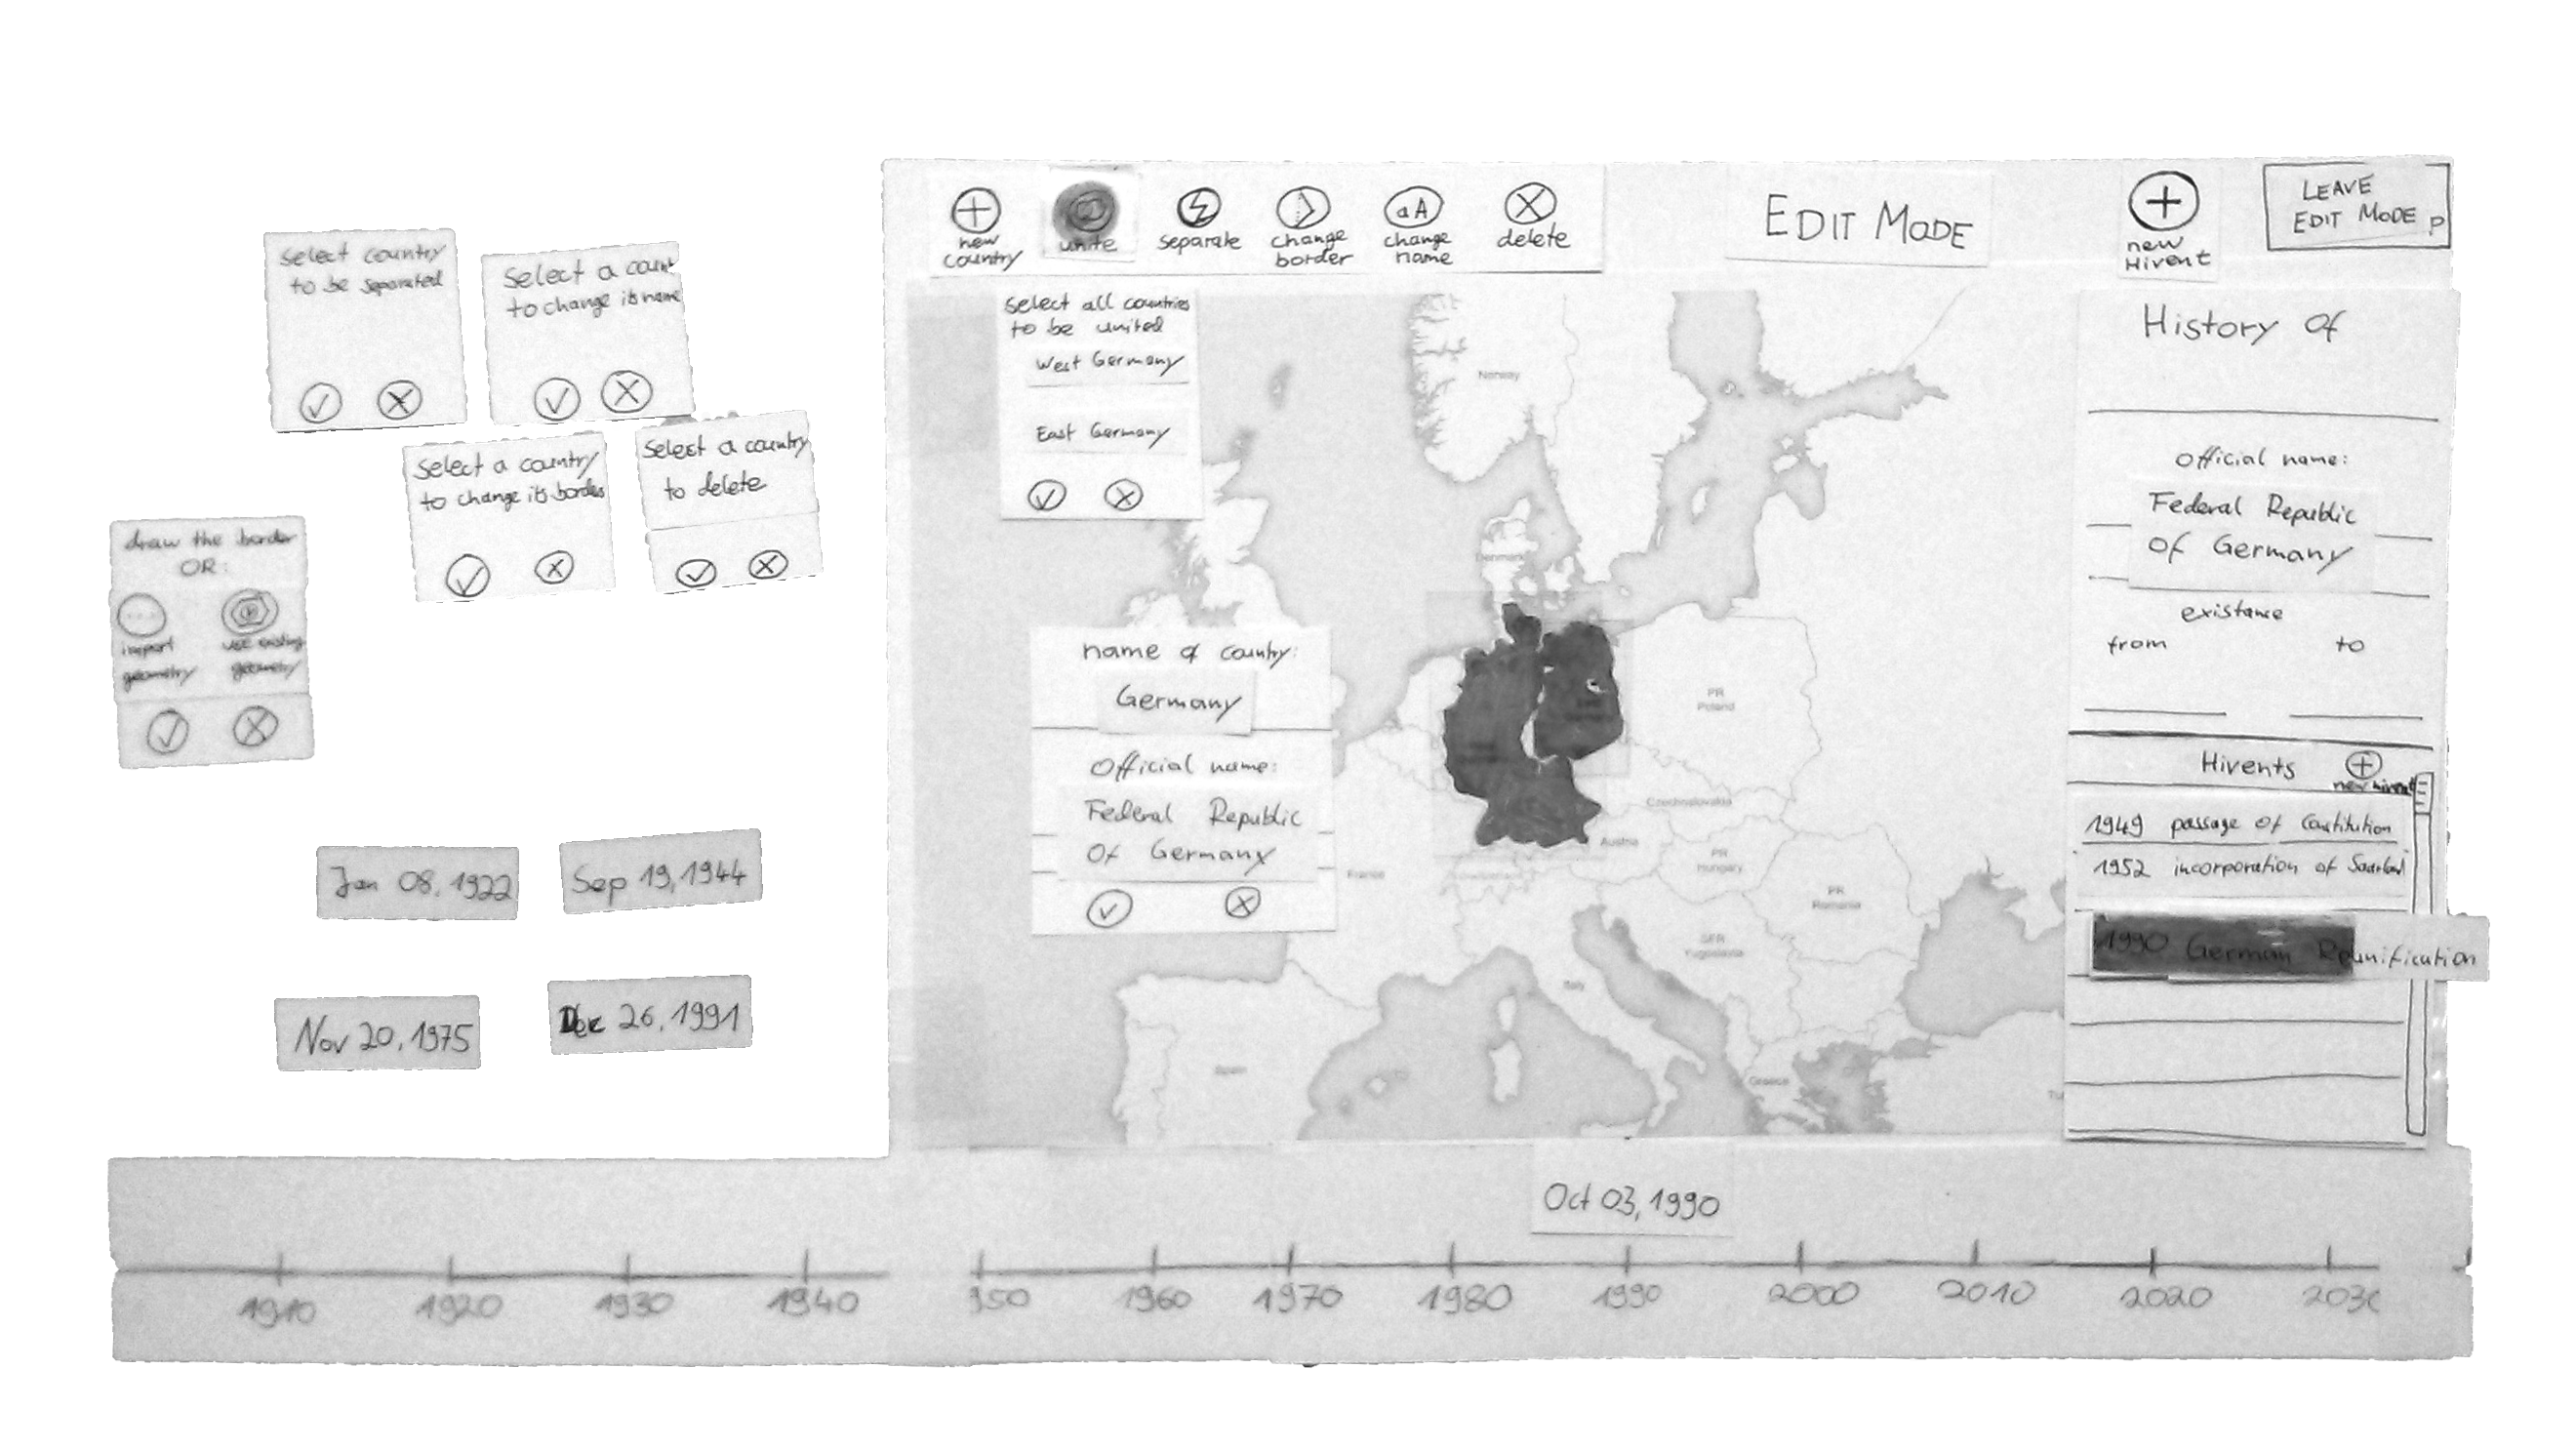
\includegraphics[width=225px]{graphics/development/design_process/paper_prototype_1.png}
\end{subfigure}%
\begin{subfigure}{.5\textwidth}
  \centering
  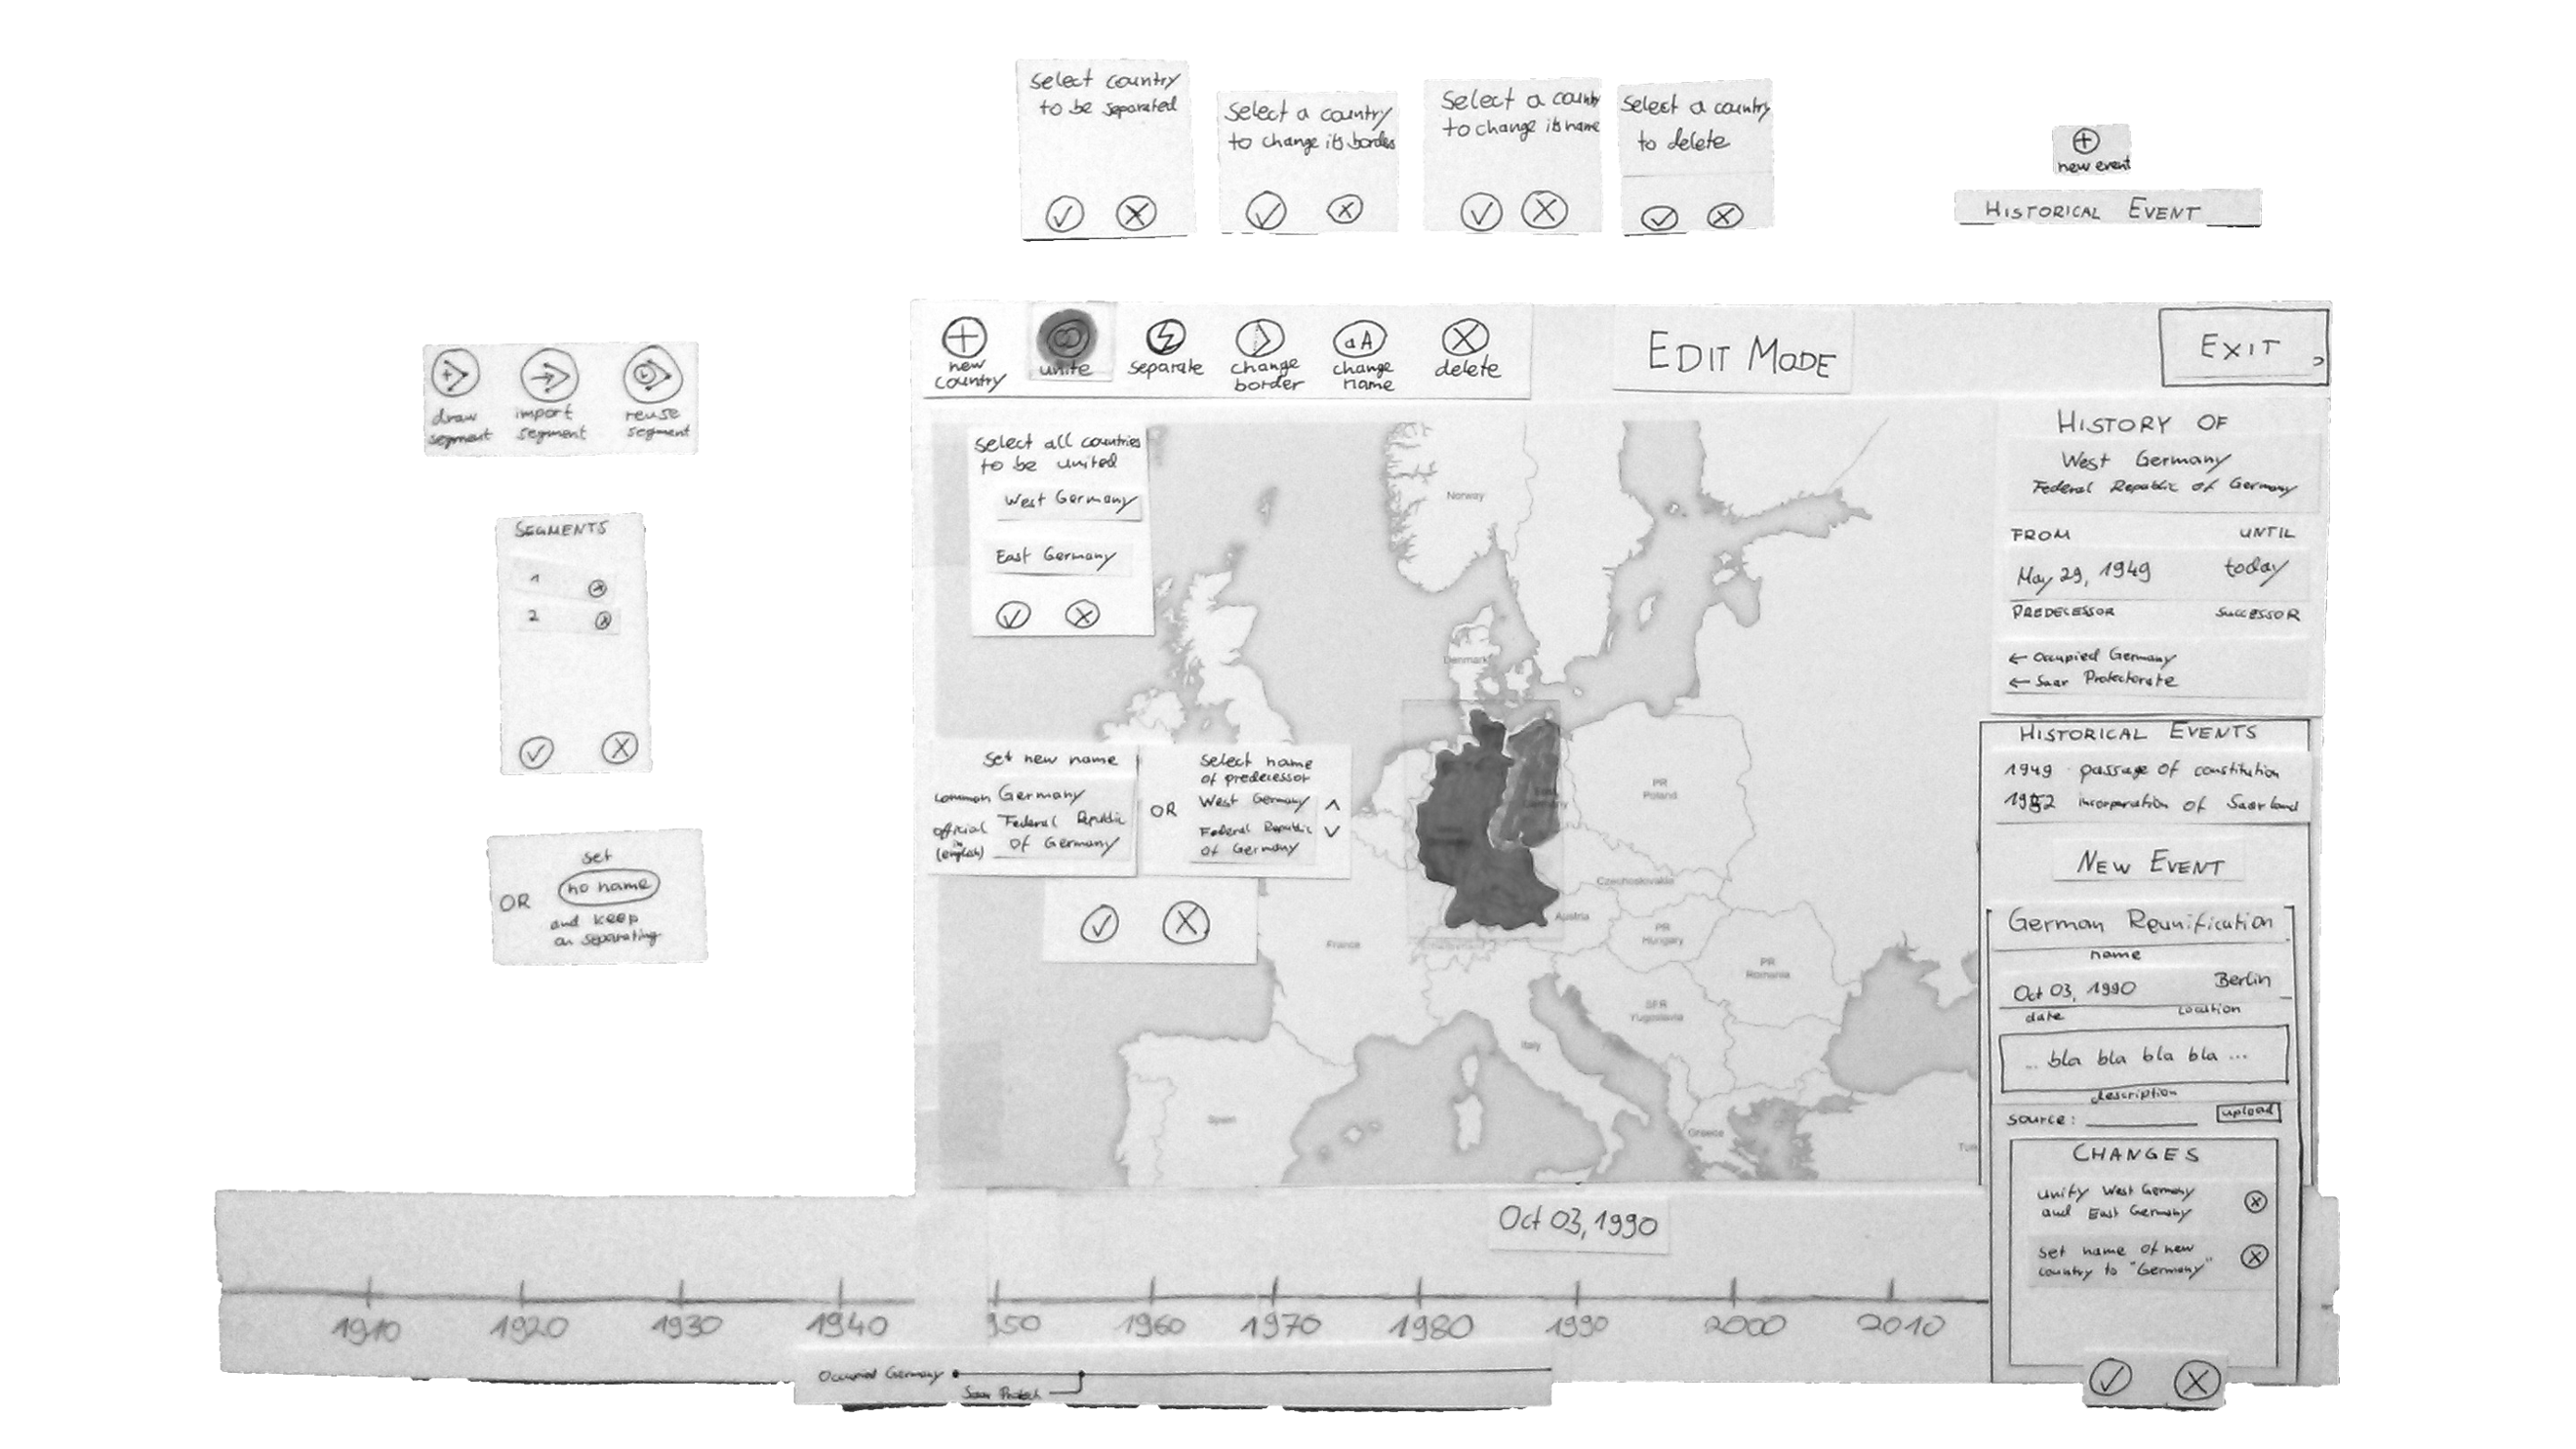
\includegraphics[width=225px]{graphics/development/design_process/paper_prototype_2.png}
\end{subfigure}
\caption{The two iteration of the paper prototype for the Edit Mode}
\label{fig:paper_prototypes}
\end{figure}

A paper prototype is very fast to create and allows to identify flaws in the concept early in the design process. Two paper prototype iterations were created in this thesis. Each iteration took about three full work days: one day to create the conceptualize and create prototype, half a day to conduct the study with three people, and one and a half days to analyze the results and rethink the concept.

Both prototypes were evaluated with three test subjects. Most parts of the interface concept were understood and all subjects could solve the first three tasks. However, there were also problems:

\begin{compactenum}
  \item There difference between Hivents, the history of a country and an historical change was unclear.
  \item The border drawing dialoge was imagined to be very complex.
  \item The backward change was not understood
  \item Correcting the name Switzerland by changing the event that created it in 1300 caused confusion.
\end{compactenum}

The main finding of this step was that depending on the task, there is both an Hivent-based and an Area-based mental model of the task. This became apparent in the German Reunification Hivent: Some users created the unification operation first, and added West and East Germany afterwards -- and some selected first West Germany, then created a unification operation and then added East Germany. From that finding arose that the interface has to support both an Hivent-based and an Area-based approach to introduce historical changes and correct information on the map.

% paragraph paper_prototype (end)

% - - - - - - - - - - - - - - - - - - - - - - - - - - - - - - - - - - - - - - -
\paragraph{Mockup Prototype} % (fold)
\label{par:mockup_prototype}

The main part of the design process was spent on the mockup prototypes. They were created in \emph{LibreOffice Impress}, an open-source slide-based presentation tool. The interface was simulated on a slide, with the map in the background, the timeline in the bottom, the set of buttons and dialogs for the Edit Mode and also the HistoGraph with geometric elements: lines, circles and rectangles. Interactivity is simulated by linking a click on a geometric element with a different slide that shows the effect of the operation. This way, sudden changes in the interface can be modelled. Creating such a mockup prototype takes longer than a paper prototype, but is still much faster than actually implementing an interactive Web-based interface. The purpose of the prototype is to rapidly develop a workflow through the interface that is understandable by the users.

\begin{figure}[H]
\centering
\begin{subfigure}[b]{.5\textwidth}
  \centering
  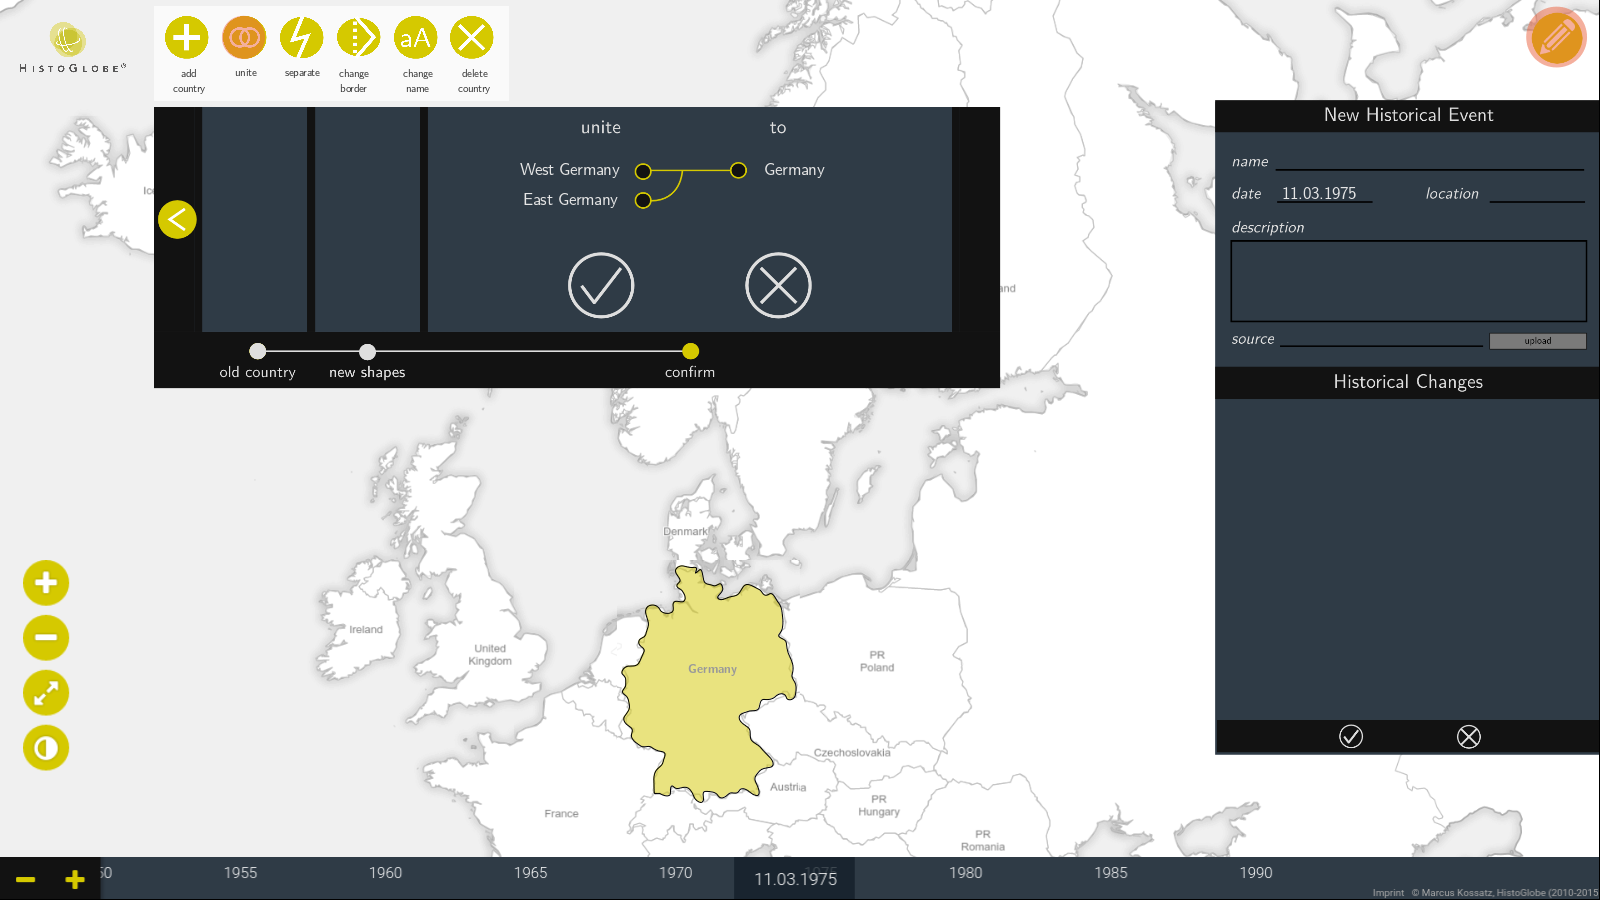
\includegraphics[width=200px]{graphics/development/design_process/mockup_prototype_1.png}
\end{subfigure}%
\begin{subfigure}[b]{.5\textwidth}
  \centering
  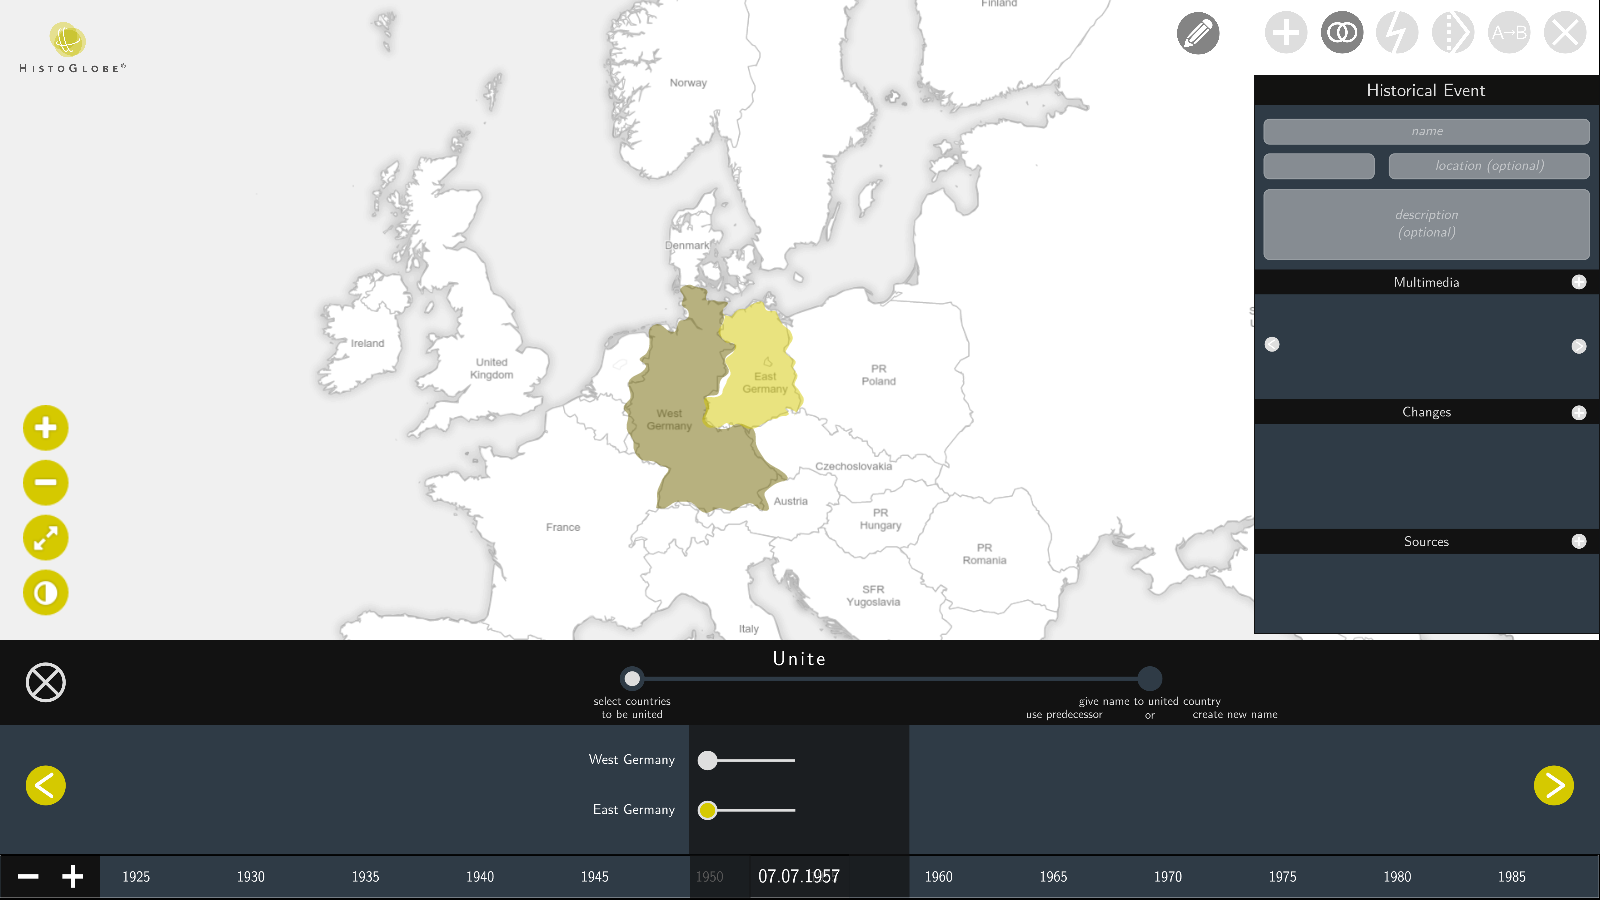
\includegraphics[width=200px]{graphics/development/design_process/mockup_prototype_2.png}
\end{subfigure} \\[0.8em]

\begin{subfigure}[b]{1.0\textwidth}
  \centering
  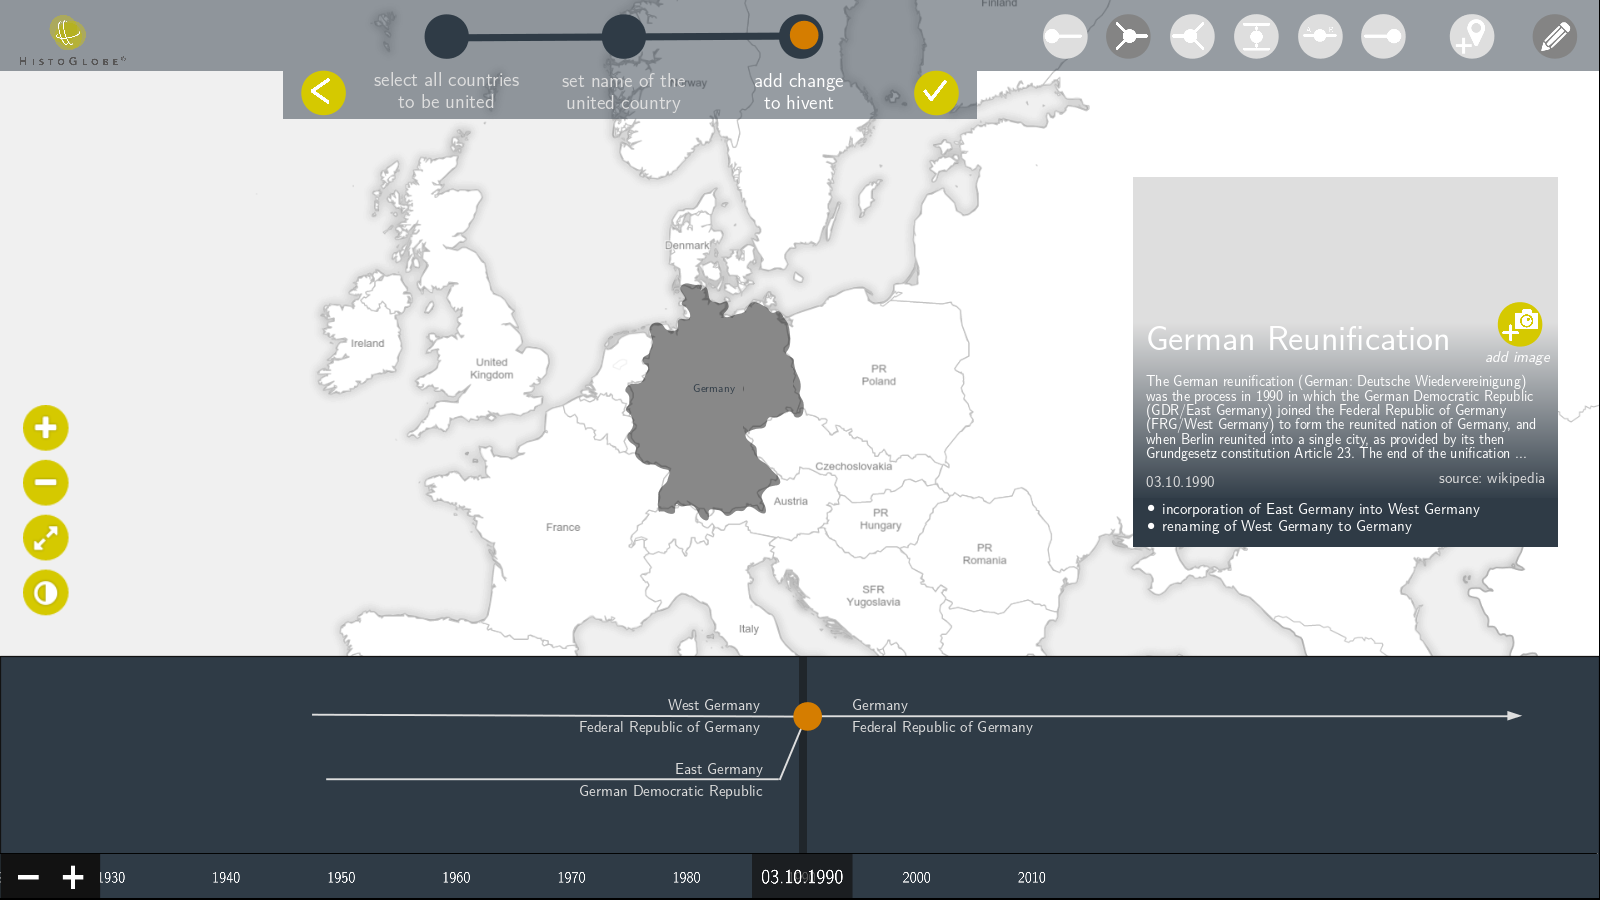
\includegraphics[width=325px]{graphics/development/design_process/mockup_prototype_3.png}
\end{subfigure}
\caption{The three iteration stages of the mockup prototype for the Edit Mode}
\label{fig:mockup_prototypes}
\end{figure}

Each prototype iteration was tested with multiple subjects and similar tasks as for the paper prototype. From one test to the next one changes to the interfaces were made. Finally, the users were able to solve all the tasks. Some interesting and partially contradicting quotes from the users were:
\begin{quoteit}
  \begin{tabular}{l r}
    ``this was much easier than I thought'' ~~~~~~~~ &
    ``there is a training session needed'' \\[0.75em]
    ``the interface is very clear &
    ``the logic makes sense, \\
    and graphically pleasing'' &
    it is just very complex'' \\[0.75em]
    ``it's looking good'' &
    ``a nice tutorial and a good \\
    & documentation are necessary'' \\
  \end{tabular}
\end{quoteit}

The main evolution was from a separate dialogue window for the Edit Operation workflow to an intergrated workflow window in the title bar. Also the HistoGraph was introduced to visualize the historical change at while editing it. A lot of smaller design issues, e.g. position of buttons, font sizes or color schemes were identified and fixed. But also concept issues arose and especially the backward change proved to be very difficult.

Three different design solutions were tested throughout the iterations and two of them proved to be promising: First of all, instead of initializing a change in 1990 to separate Germany into East and West, the user can introduce two creation events for the two German states in May and October 1949. The interface needs to provide a visual clue that after creating West Germany, this Area can only be active until 1990, because then another Area, present-day Germany, uses its territory (see figure \ref{sfig:backward_change_1}). The change from West Germany to Germany will be created automatically. The second approach is to introduce a button that flippes an Edit Operation that has just been created (see figure \ref{sfig:backward_change_2}) -- in this case the \texttt{DIS} operation introduced to secede East Germany from Germany will be flipped into a \texttt{UNI} operation to incorporate East Germany into Germany. This approach makes use of the fact that each Edit Operation and therefore also each underlying HG Operation has an inverse.
% TODO: reference to inverse?
However, this flipping requires the introduction of additional creation events: West and East Germany were introduced in the change, but only the event that ceases both of them (\texttt{INC} of West Germany into East Germany). They also need a creation event, otherwise they would be active backwards all the way to $t_0$, the initial state of the system.

\begin{figure}[H]
\centering
\begin{subfigure}[b]{.5\textwidth}
  \centering
  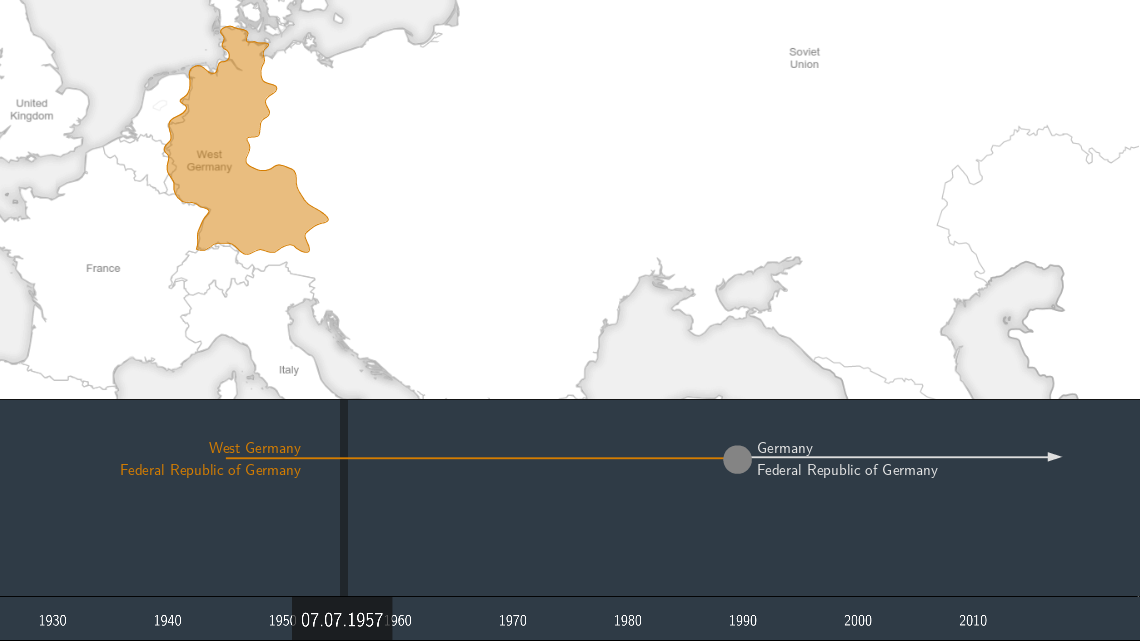
\includegraphics[width=200px]{graphics/development/design_process/backward_change_1.png}
  \caption{Visual clue: predefined and of Area}
  \label{sfig:backward_change_1}
\end{subfigure}%
\begin{subfigure}[b]{.5\textwidth}
  \centering
  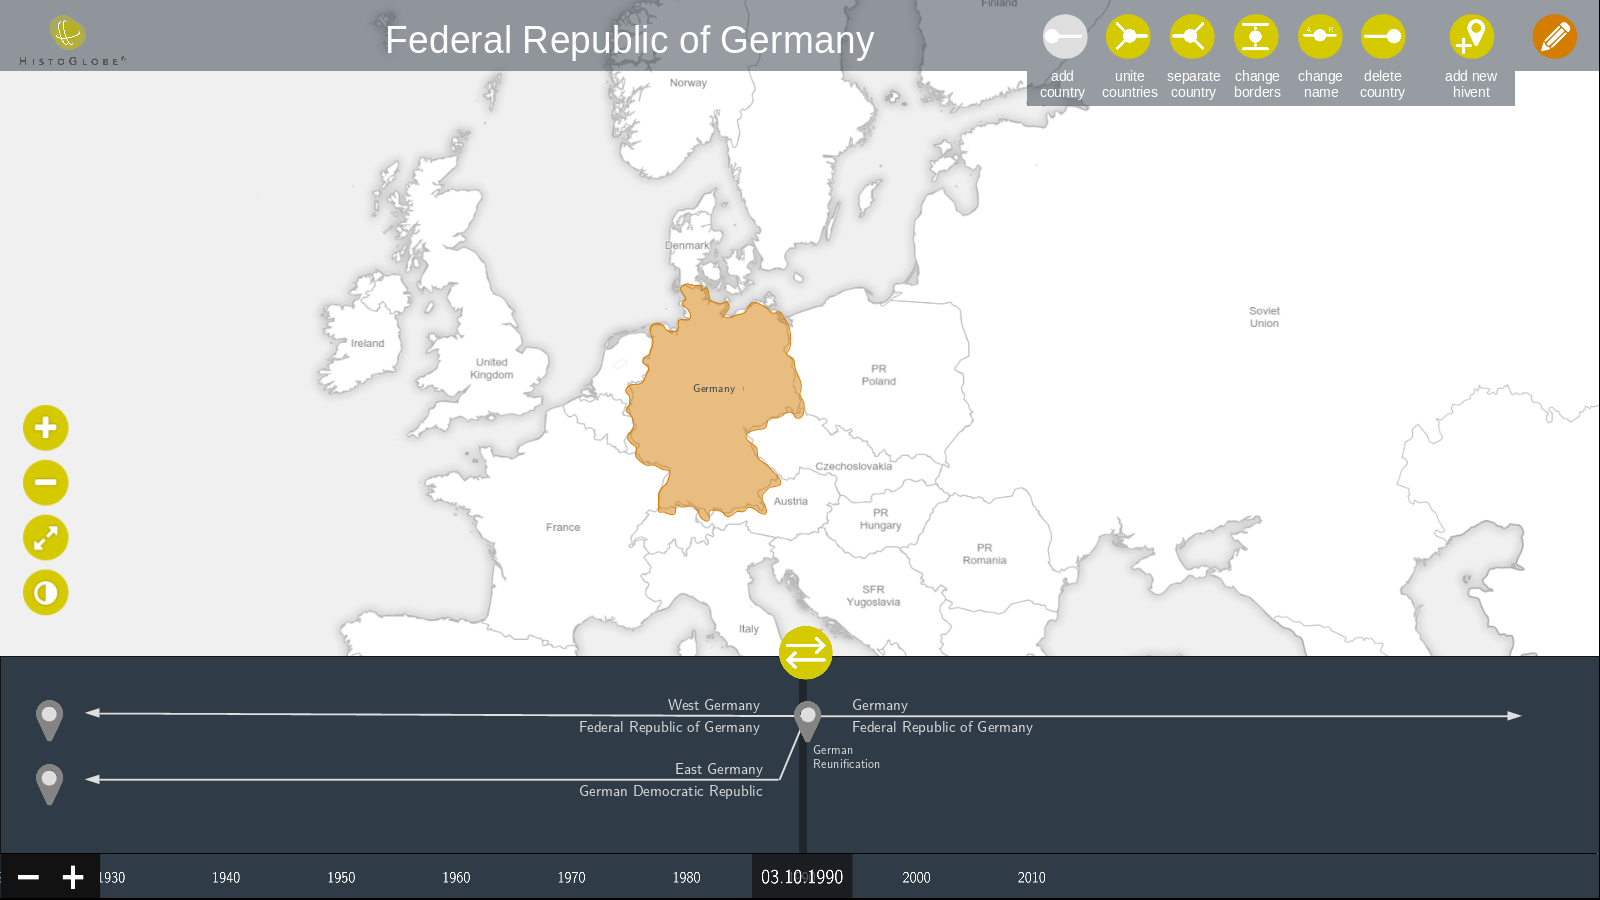
\includegraphics[width=200px]{graphics/development/design_process/backward_change_2.png}
  \caption{Create backward change by flipping Edit Operation}
  \label{sfig:backward_change_2}
\end{subfigure}
\caption{Two approaches for editing changes backwards}
\label{fig:backward_change}
\end{figure}

The prototype proved to be very valuable for the development process. In a total of two weeks, an interface concept and workflow was designed that proved to be understandable by the users.


% paragraph mockup_prototype (end)

% - - - - - - - - - - - - - - - - - - - - - - - - - - - - - - - - - - - - - - -
\paragraph{Final Web-based prototype} % (fold)
\label{par:final_web_based_prototype}

The main advantage of the design process is that it prevents major redesigns of the final Web-based prototype. After three months of implementation of the final system, the interface looks very similar to the last version of the mockup prototype.

The original main elements of the interface are the map, the timeline with the Now Marker indicating the current date of the visualization and the control buttons for zooming the map and the timeline. They are preserved and extended by new interface elements for the Edit Mode. Their interaction and behavior are introduced in this section at the example of the fictional secession of Scotland from the United Kingdom in 2018. The HistoGraph was not implemented, because of the conceptual problems mentioned in section \ref{sub:histograph} that have to be solved first.


\begin{minipage}[t]{0.47\textwidth}

  \begin{figure}[H]
    \centering
    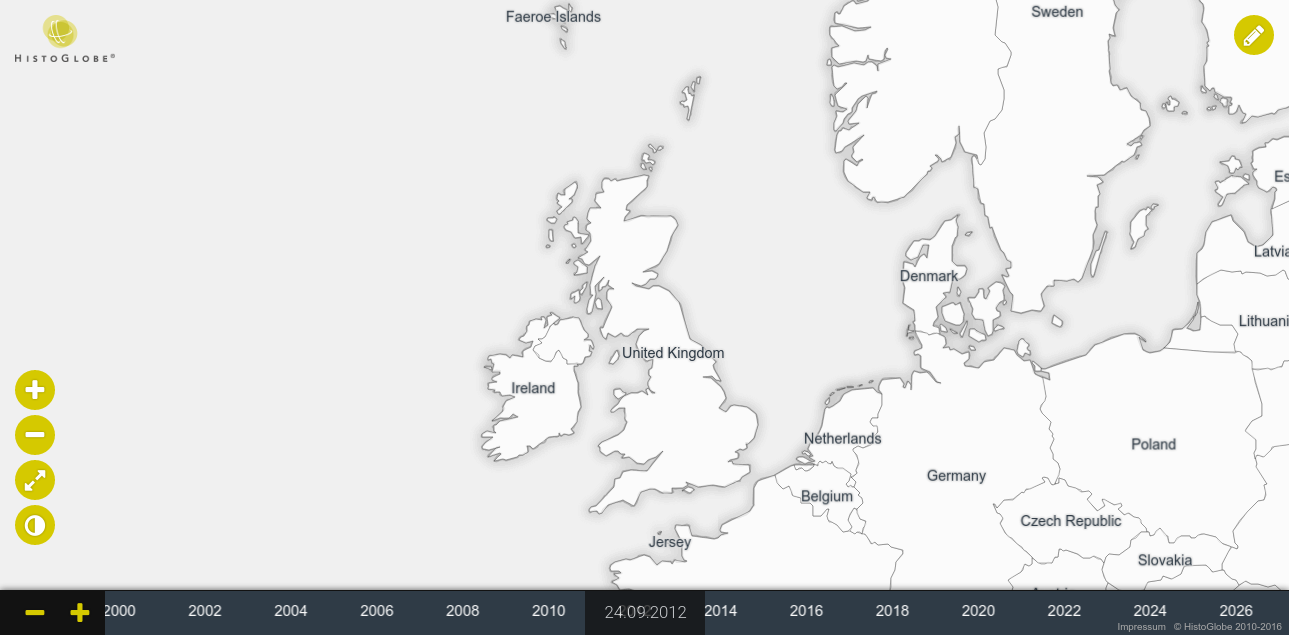
\includegraphics[width=1.0\textwidth]{graphics/development/final_interface/1_init.png}
    \caption{Initial state of the normal mode}
    \label{fig:final_1_init}
  \end{figure}

  The initial state of the user interface. Additional to the original elements, there is an edit button on the upper right corner. Clicking it enters the Edit Mode of the system.

\end{minipage}    % N.B. the % is very important
\hspace{1.5em}    % N.B. this must go in this line, no blank lines !!!
\begin{minipage}[t]{0.47\textwidth}

  \begin{figure}[H]
    \centering
    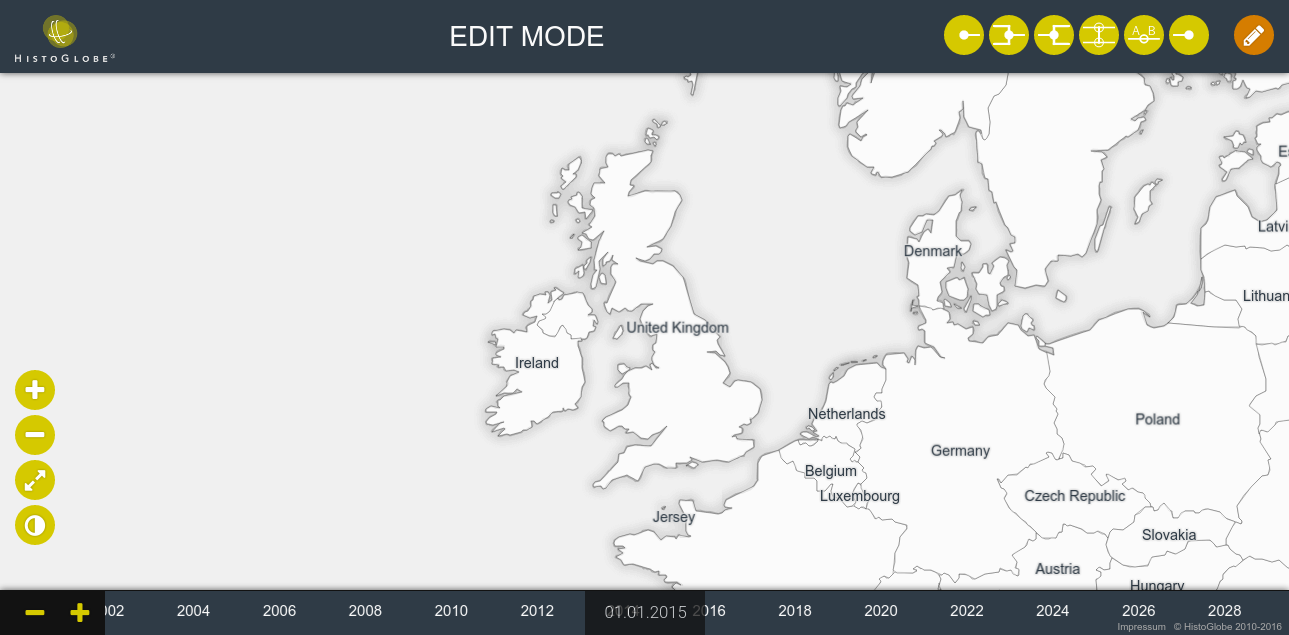
\includegraphics[width=1.0\textwidth]{graphics/development/final_interface/2_edit_mode.png}
    \caption{Initial state of the Edit Mode}
    \label{fig:final_2_edit_mode}
  \end{figure}

  In the Edit Mode, a title bar and six buttons for the Edit Operations are   revealed. Clicking a button starts the operation workflow introduced in section \ref{par:workflow}.

\end{minipage}

\vspace{1em}
\begin{minipage}[t]{0.47\textwidth}

  \begin{figure}[H]
    \centering
    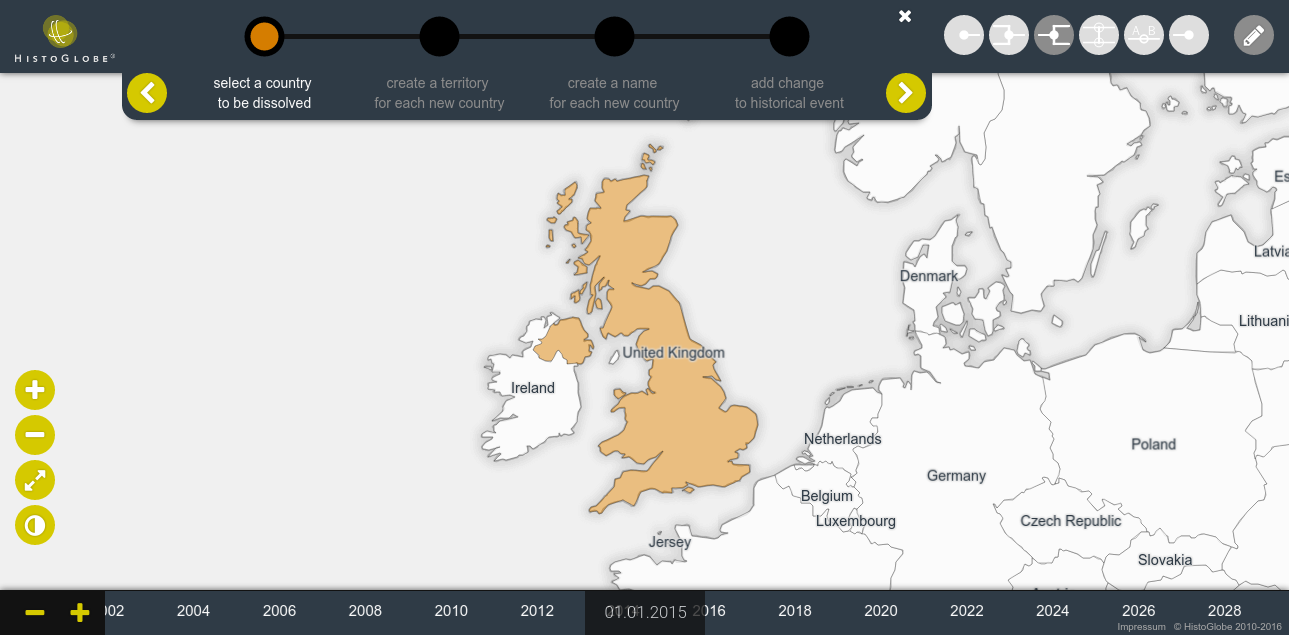
\includegraphics[width=1.0\textwidth]{graphics/development/final_interface/3_select_old_areas.png}
    \caption{Step 1) \texttt{SELECT\_OLD\_AREAS}}
    \label{fig:final_3_select_old_areas}
  \end{figure}

  A \emph{Workflow Window} is guiding the user through the process of completing the historical change. It shows all the steps necessary for this Edit Operation. In the case of \texttt{DIS}, the user has to select the country to be dissolved by clicking it on the map. After the step is completed, clicking the next button in the workflow window procceeds to the next step. At each point in the workflow, clicking the back button reverts the previous action.

\end{minipage}    % N.B. the % is very important
\hspace{1.5em}    % N.B. this must go in this line, no blank lines !!!
\begin{minipage}[t]{0.47\textwidth}

  \begin{figure}[H]
    \centering
    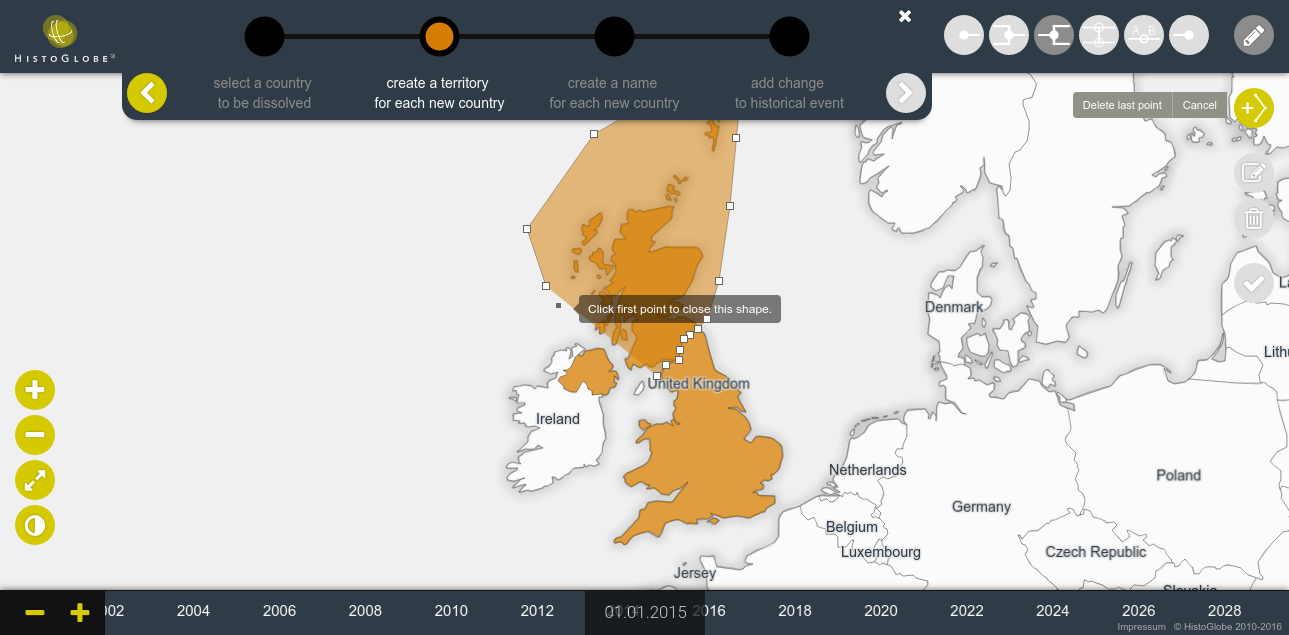
\includegraphics[width=1.0\textwidth]{graphics/development/final_interface/4_set_new_territories.png}
    \caption{step 2) \texttt{SET\_NEW\_TERRITORIES}}
    \label{fig:final_4_set_new_territories}
  \end{figure}

  In the second step, the user has to create the territory for each new Area that shall be created. Therefore, the \emph{New Territory Tool} provides the functionality to create, manipulate and delete polylines by clicking and moving it directly on the map. The polypolygon drawn by the user is intersected with the old territory to create the territory of the new Area. After one new territory is created sucessfully, the second one can be taken from the remaining old territory by selecting it from the map. As soon as the whole old territory is distributed among the new Areas, the workflow proceeds to the next step.

\end{minipage}

\vspace{1em}
\begin{minipage}[t]{0.47\textwidth}

  \begin{figure}[H]
    \centering
    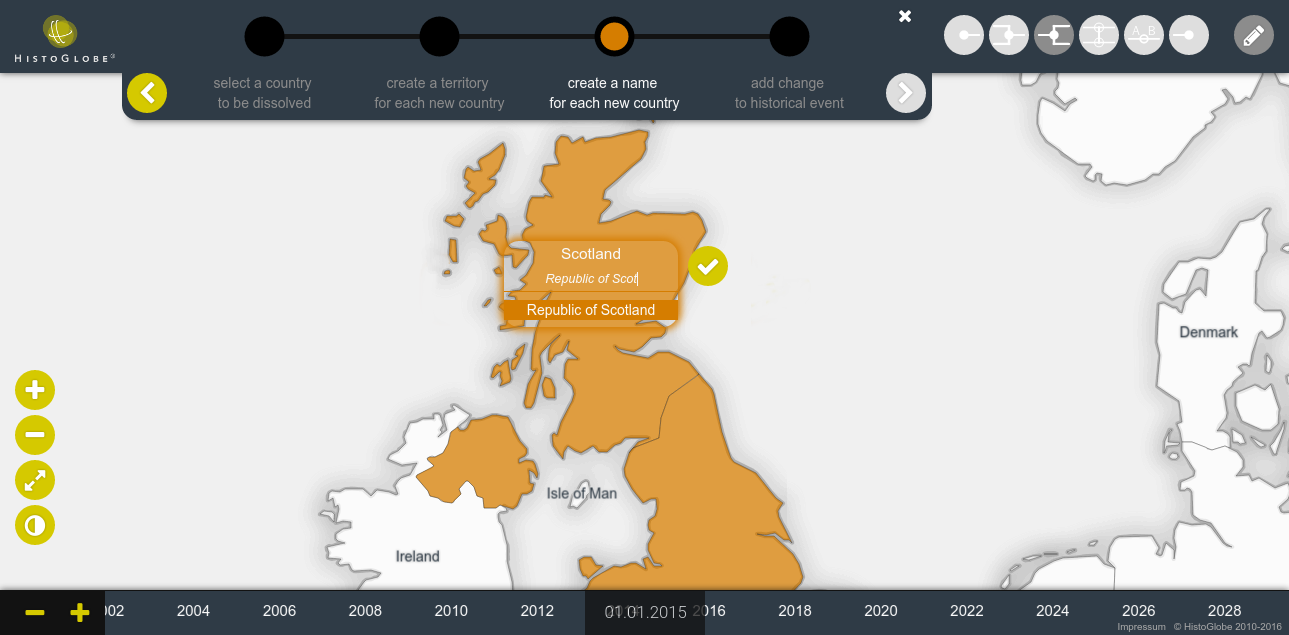
\includegraphics[width=1.0\textwidth]{graphics/development/final_interface/5_set_new_name.png}
    \caption{Step 3) \texttt{SET\_NEW\_NAMES}}
    \label{fig:final_5_set_new_name}
  \end{figure}

  In the next step, for each Area that has been created in the step before, a name has to be defined. The \emph{New Name Tool} is a draggable input form with two lines, the upper one for the short name, the lower one for the formal name, the identity of the Area. Via instant search, the user can select existing country names from the database to be put in the New Name Tool. When clicking the confirm button, the short name is put directly on the map.

\end{minipage}    % N.B. the % is very important
\hspace{1.5em}    % N.B. this must go in this line, no blank lines !!!
\begin{minipage}[t]{0.47\textwidth}

  \begin{figure}[H]
    \centering
    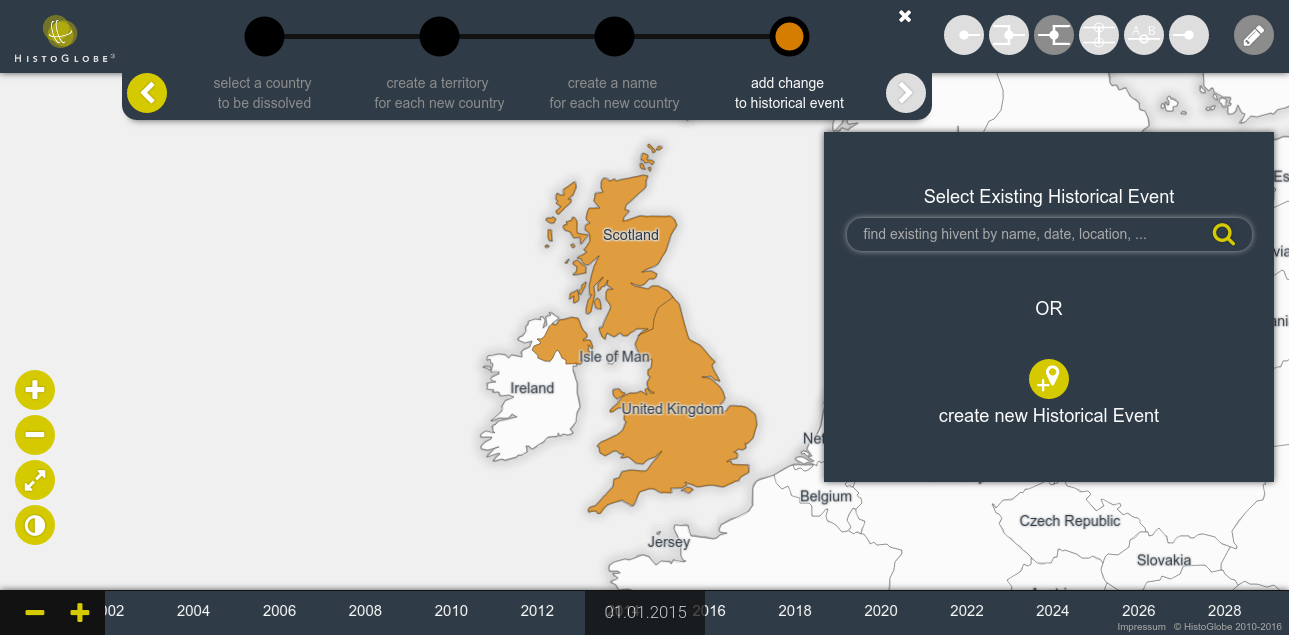
\includegraphics[width=1.0\textwidth]{graphics/development/final_interface/6_add_change_to_hivent_1.png}
    \caption{Step 4) \texttt{ADD\_CHANGE}}
    \label{fig:final_6_add_change_to_hivent_1}
  \end{figure}

  When all names are set, the Edit Operation is complete. In the last step of the workflow, it has to be added to an Hivent. The \emph{New Hivent Box} offers two possibilities: the user can search for an existing Hivent and add the historical change to it, or create a new one.

\end{minipage}

\vspace{1em}
\begin{minipage}[t]{0.47\textwidth}

  \begin{figure}[H]
    \centering
    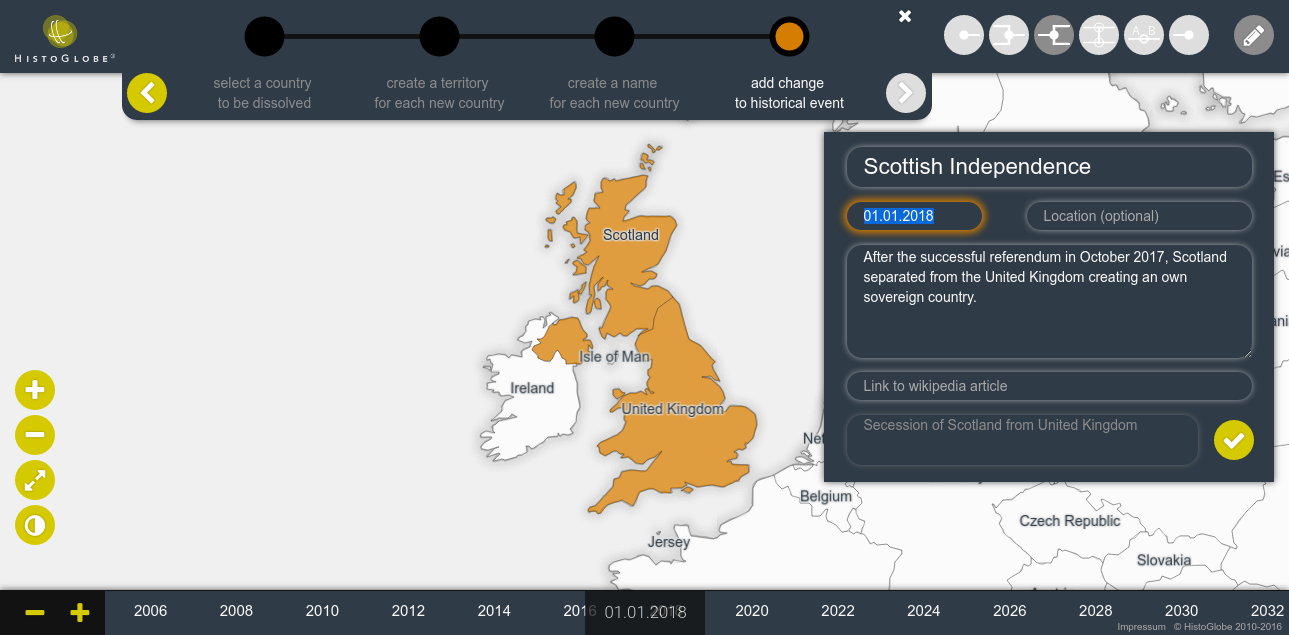
\includegraphics[width=1.0\textwidth]{graphics/development/final_interface/7_add_change_to_hivent_2.png}
    \caption{Step 4) \texttt{ADD\_CHANGE}}
    \label{fig:final_7_add_change_to_hivent_2}
  \end{figure}

  The new Hivent created for that change is the ``Scottish Independence'' on 01.01.2018 with a description of the Hivent and possibly a location and a link to a wikipedia article. In the last line, the historical change ``Secession of Scotland from the United Kingdom'' is noted. Clicking the confirm button finalizes the workflow.

\end{minipage}    % N.B. the % is very important
\hspace{1.5em}    % N.B. this must go in this line, no blank lines !!!
\begin{minipage}[t]{0.47\textwidth}

  \begin{figure}[H]
    \centering
    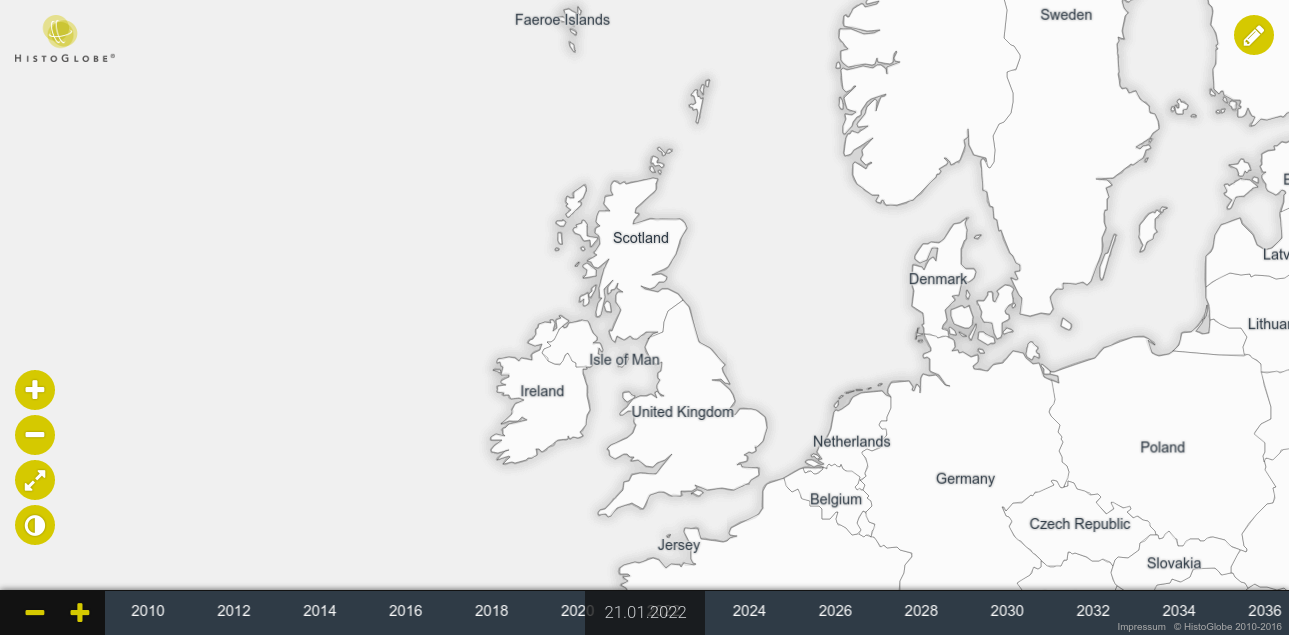
\includegraphics[width=1.0\textwidth]{graphics/development/final_interface/8_final_state.png}
    \caption{The final state with Scotland}
    \label{fig:final_8_final_state}
  \end{figure}

  Clicking the edit button again leaves the Edit mode back to the normal view. Scotland and the United Kingdom are both visible on the map after 2018. When moving the timeline before 2018, Scotland is still part of the UK.

\end{minipage}

% paragraph final_web_based_prototype (end)

% subsection design_iterations (end)

% section histoglobe_interface (end)
%!TEX root = ../masters_thesis.tex

\section{HistoGlobe Application} % (fold)
\label{sec:histoglobe_application}

- the final version of the application behind the interface built on top of the data model

distributed Web-based system
classic approach: UI <-> Client (main program) <-> Server (middleware) <-> DB

problems
- backward change: all HG Operations and Edit Operations are inversible :)
- support uncertainty

% ------------------------------------------------------------------------------
\subsection{System Architecture} % (fold)
\label{sub:system_architecture}


The system developed in this thesis is Web-based. That means, there is a \emph{client}, a Web browser, and a remote Web \emph{server} with a database and a middleware. The Web browser hosts the applications user interface. If the user interacts with a tool the client sends a request to the Web server for new data. The middleware checks the request and queries the necessary data from the database. The data will be transformed and sendt back to the client. On the map and the timeline the new information will be shown.

This clear separation between the data (\emph{model}), the user interface (\emph{view}) and the middleware (\emph{controller}) follows directly from the \emph{model-view-controller pattern}: One part can be changed without interfering the other parts, e.g. if the 2D map is replaced by a 3D globe, only the view changes, but the middleware and the database can stay untouched. Likewise, the implementation of a new database technology has no consequences to the view.

graphic of basic system:
UI
Client-side mechanism
Server-side mechanism
Database

programming languages / Framworks
Client                    HTML
          Less ->         CSS
          CoffeeScript -> JavaScript
Server    Django ->       Python
                          PostgreSQL
                          + PostGIS

% subsection system_architecture (end)

% ------------------------------------------------------------------------------
\subsection{Database Model} % (fold)
\label{sub:database_model}

database model

\begin{compactenum}
  \item The \emph{name} of the Hivent.
  \item A textual \emph{description} of the topic of the Hivent.
  \item The point in time, identified by the Hivent \emph{date}.
  \item The Hivent \emph{location}.
  \item The \emph{historical changes} resulting from the Hivent.
\end{compactenum}


           Hivent
             m
       HistoricalChange
             m
  --------AreaChange------
  |          |           |
  |     ----Area----     |
  m     m          m     m
AreaTerritory      AreaName

no transaction time, only valid / event time
only world time is regarded, not database time.

view

get\_all
save\_operation

% subsection database_model (end)


% ------------------------------------------------------------------------------
\subsection{Computational Model} % (fold)
\label{sub:computational_model}

Class diagram

HistoGlobe

SpatialDisplay -> Map

TimeController  <-> Timeline
                <-> NowMarker

HiventController                AreaController <->  AreasOnMap
HiventHandle                    AreaHandle
Hivent
HistoricalChange    AreaChange  Area
                                AreaName            AreaNameLayerOnMap
                                AreaTerritory       AreaTerritoryLayerOnMap

DatabaseInterface

EditMode -> EditOperation -> EditOperationStep
NewTerritoryTool* NewNameTool NewHiventBox
WorkflowWindow

HistoGraph

LabelManager*

important little utils
  Button, ButtonArea
  NumberInput, TextInput, TextInputArea
  Title
  Watermark
  DoublyLinkedList
  WithinTree
  Geometry -> Polypolygon -> Polygon -> Polyline -> Point

% - - - - - - - - - - - - - - - - - - - - - - - - - - - - - - - - - - - - - - -
\paragraph{Reduction to HG Operations} % (fold)
\label{par:reduction_to_hg_operations}

% wording:
% UNI of "[old]"  to    "new"
% INC of "[old]"  into  "pres"
% SEP of "old"    into  "[new]"
% SEC of "[new]"  from  "pres"
% NCH of "pres"

Each Edit Operation will internally be expressed by a set of Historical Geographic Operations that describe the change on a low level. Depending on the input of the user in the Edit Operation steps, there are different possibilities. They are introduced in table \ref{tab:editoperations_to_hg_operations}.

\begin{center}
\begin{longtable}{m{1.2cm} m{0.95cm} m{0.95cm} m{0.95cm} m{6.0cm} m{2.3cm}}
  \toprule

  \pbox{1.2cm}{EditOp.\\(case)} &
  \pbox{0.95cm}{old\\Areas\\[-0.8em]} &
  \pbox{0.95cm}{update\\Areas\\[-0.8em]} &
  \pbox{0.95cm}{new\\Areas\\[-0.8em]} &
  expression by HG Operations \protect\footnotemark &
  visualization \\
  \midrule
  \endhead

  % TODO: introduce T as territory that is used like a temporary Area with exactly that territoy
  % CREATE

  \multirow{9}{*}{\texttt{CRE} (1)} &
  \multicolumn{4}{p{10cm}}{
    Area $B_1$ is created with territory $T$. The part of $T$ that is on previously unclaimed land ($T_\Omega$) is seceded as $B_1$ from $\Omega$.
    If $T_\Omega$ is empty, then $B_1$ is initialized with an empty territory.
    The rest of $T$ covers some Areas $A_p$ partially and some Areas $A_f$ fully.
    For each $A_p$, the covered territory $T_p$ is seceded and incorporated into $B_1$.
    Each $A_f$ is completely incorporated into $B_1$.
  } &
  \multirow{9}{*}{
    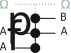
\includegraphics[width=2.5cm]{graphics/development/edit_to_hg_operations/CRE_to_SEC+UNI}
  } \\

  &
  $n_f$ &
  $n_p$ &
  $1$ &
  \pbox{6.0cm}{
    ~\\
    \texttt{SEC} of $B_1$ from $\Omega$ \\
    \texttt{SEC} of $T_p$ from $A_p$, \texttt{INC} of $T_p$ into $B_1$ \\
    \texttt{INC} of $A_f$ into $B_1$
  } &
  \\

  % MERGE
  \midrule
  \multirow{3}{*}{\texttt{MRG} (1)} &
  \multicolumn{4}{p{10cm}}{
    Multiple Areas $A_i$ are unified to $B_1$. The new Area receives a new name distinct from all the names of $A_i$.
  } &
  \multirow{3}{*}{
    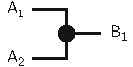
\includegraphics[width=2.5cm]{graphics/development/edit_to_hg_operations/MRG_to_UNI}
  } \\
  &
  $n \geq 2$ &
  $0$ &
  $1$ &
  \pbox{6.0cm}{
    ~\\
    \texttt{UNI} of $\forall A_i$ to $B_1$
  } &
  \\

  \midrule
  \multirow{4}{*}{\texttt{MRG} (2)} &
  \multicolumn{4}{p{10cm}}{
    Multiple Areas $A_i$ are unified, the resulting Area reuses the short and formal name of one of the old Areas ($A_p$) and therefore preserves it. The remaining Areas $A_i$ are incorporated into $A_p$.
  } &
  \multirow{4}{*}{
    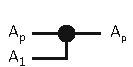
\includegraphics[width=2.5cm]{graphics/development/edit_to_hg_operations/MRG_to_INC}
  } \\
  &
  $n \geq 1$ &
  $1$ &
  $1$ &
  \pbox{6.0cm}{
    ~\\
    \texttt{INC} of $\forall A_i$ into $A_p$
  } &
  \\

  \midrule
  \multirow{4}{*}{\texttt{MRG} (3)} &
  \multicolumn{4}{p{10cm}}{
    The same as the previous case, just that $A_p$ receives a new short name and therefore an additional name change is required.
  } &
  \multirow{4}{*}{
    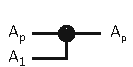
\includegraphics[width=2.5cm]{graphics/development/edit_to_hg_operations/MRG_to_INC+NCH}
  } \\
  &
  $n \geq 1$ &
  $1$ &
  $1$ &
  \pbox{6.0cm}{
    ~\\
    \texttt{INC} of $\forall A_i$ into $A_p$ \\
    \texttt{NCH} of $A_p$
  } &
  \\

  % DISSOLVE

  \midrule
  \multirow{4}{*}{\texttt{DIS} (1)} &
  \multicolumn{4}{p{10cm}}{
    Separate one Area $A_1$ into multiple new Areas $B_i$ and define a territory and name for each of them. Each name is distinct from the name of the old Area.
  } &
  \multirow{4}{*}{
    
\includegraphics[width=2.5cm]{graphics/development/edit_to_hg_operations/DIS_to_SEP}
  } \\
  &
  $1$ &
  $0$ &
  $n \geq 2$ &
  \pbox{6.0cm}{
    ~\\
    \texttt{SEP} of $A_1$ into $\forall B_i$
  } &
  \\

  \midrule
  \multirow{5}{*}{\texttt{DIS} (2)} &
  \multicolumn{4}{p{10cm}}{
    Separate multiple Areas $B_1$ from one initial Area $A_p$ and define a territory and name for each of them. One of the separated Areas has the same short and formal name as $A_p$, so it continues its identity and preserves the Area. The remaining new Areas secede from $A_p$.
  } &
  \multirow{5}{*}{
    
\includegraphics[width=2.5cm]{graphics/development/edit_to_hg_operations/DIS_to_SEC}
  } \\
  &
  $1$ &
  $1$ &
  $n \geq 1$ &
  \pbox{6.0cm}{
    ~\\
    \texttt{SEC} of $\forall B_i$ from $A_p$
  } &
  \\

  \midrule
  \multirow{4}{*}{\texttt{DIS} (3)} &
  \multicolumn{4}{p{10cm}}{
    The same as the previous case, just that $A_p$ receives a new short name and therefore an additional name change is required.
  } &
  \multirow{4}{*}{
    
\includegraphics[width=2.5cm]{graphics/development/edit_to_hg_operations/DIS_to_SEC+NCH}
  } \\
  &
  $1$ &
  $1$ &
  $n \geq 1$ &
  \pbox{6.0cm}{
    ~\\
    \texttt{SEC} of $\forall B_i$ from $A_p$  \\
    \texttt{NCH} of $A_p$
  } &
  \\

  % CHANGE BORDER

  \midrule
  \multirow{10}{*}{\texttt{CHB} (1)} &
  \multicolumn{4}{p{10cm}}{
    One existing Area $A_1$ is selected and its territory changes. Relative to the old territory some parts of the territory expanded ($T_e$) and some withdrew ($T_w$).
    The part of $T_e$ that expanded into unclaimed land ($T_\Omega \in T_e$) is seceded from $\Omega$ and incorporated into $A_1$.
    The Areas $A_f$ fully covered by $T_e$ are incorporated into $A_1$,
    the Areas $A_p$ partially covered by $T_e$ secede this territory $T_p \in T_e$ to $A_1$.
    $T_w$ will be incorporated into $\Omega$, resulting in unclaimed land.
  } &
  \multirow{10}{*}{
    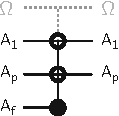
\includegraphics[width=2.5cm]{graphics/development/edit_to_hg_operations/CHB_to_SEC+INC_omega}
  } \\
  &
  $n_f$ &
  $1+n_p$ &
  $0$ &
  \pbox{6.0cm}{
    ~\\
    \texttt{SEC} of $T_\Omega$ from $\Omega$,
    \texttt{INC} of $T_\Omega$ into $A_1$ \\
    \texttt{SEC} of $T_p$ from $A_p$,
    \texttt{INC} of $T_p$ into $B_1$ \\
    \texttt{INC} of $A_f$ into $B_1$ \\
    \texttt{SEC} of $T_w$ from $B_1$,
    \texttt{INC} of $T_w$ into $\Omega$
  } &
  \\

  \midrule
  \multirow{7}{*}{\texttt{CHB} (2)} &
  \multicolumn{4}{p{10cm}}{
    Two existing Areas $A_1$ and $A_2$ are selected and their common border changes. This results in a symmetrical change of territories, made up by two sets of territories: $T_2$ that previously belonged to $A_1$ and is now part of $A_2$ and $T_1$ for which the opposite is true. $T_2$ is seceded by $A_1$ and incorporated into $A_2$, the opposite happenes to $T_1$.
  } &
  \multirow{7}{*}{
    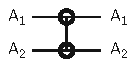
\includegraphics[width=2.5cm]{graphics/development/edit_to_hg_operations/CHB_to_SEC+INC}
  } \\
  &
  $0$ &
  $2$ &
  $0$ &
  \pbox{6.0cm}{
    ~\\
    \texttt{SEC} of $T_2$ from $A_1$,
    \texttt{INC} of $T_2$ into $A_2$ \\
    \texttt{SEC} of $T_1$ from $A_2$,
    \texttt{INC} of $T_1$ into $A_1$
  } &
  \\

  % RENAME

  \midrule
  \multirow{3}{*}{\texttt{REN} (1)} &
  \multicolumn{4}{p{10cm}}{
    One Area $A_1$ is selected and both its short and formal name is changed. Therefore, a new Area $B_1$ is created as a direct successor of $A_1$. This is a special case of a unification with only one Area.
  } &
  \multirow{3}{*}{
    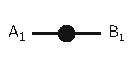
\includegraphics[width=2.5cm]{graphics/development/edit_to_hg_operations/REN_to_UNI}
  } \\
  &
  $1$ &
  $0$ &
  $1$ &
  \pbox{6.0cm}{
    \texttt{UNI} of $A_1$ to $B_1$
  } &
  \\

  \midrule
  \multirow{3}{*}{\texttt{REN} (2)} &
  \multicolumn{4}{p{10cm}}{
    One Area $A_1$ is selected and receives a new short name, but the formal name and therefore the identity is preserved. $A_1$ is updated.
  } &
  \multirow{3}{*}{
    
\includegraphics[width=2.5cm]{graphics/development/edit_to_hg_operations/REN_to_NCH}
  } \\
  &
  $0$ &
  $1$ &
  $0$ &
  \pbox{6.0cm}{
    \texttt{NCH} of $A_1$
  } &
  \\

  % CEASE

  \midrule
  \multirow{2}{*}{\texttt{CES} (1)} &
  \multicolumn{4}{p{10cm}}{
    One Area $A_1$ is selected and ceases by incorporating into the universe.
  } &
  \multirow{2}{*}{
    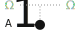
\includegraphics[width=2.5cm]{graphics/development/edit_to_hg_operations/CES_to_INC}
  } \\
  &
  $1$ &
  $0$ &
  $0$ &
  \pbox{6.0cm}{
    \texttt{INC} of $A_1$ into $\Omega$
  } &
  \\

  \bottomrule
\caption{Translation from Edit Operations to HG Operations}
\end{longtable}
\label{tab:editoperations_to_hg_operations}
\end{center}
\footnotetext{multiple HG Operations in one row happen exactly at the same time point, so they are combined}

% paragraph reduction_to_hg_operations (end)

% - - - - - - - - - - - - - - - - - - - - - - - - - - - - - - - - - - - - - - -
\paragraph{Functional description} % (fold)
\label{par:functional_description}

Each HG Operation can be described by a mathematical function. The following symbols are used in the equations:

\begin{addmargin}[1em]{0em}
\begin{tabbing}
  symbolxx \= description1xx \= description2 \kill
  $A$ \> set of old Areas that were active before the Historical Change \\
  $B$ \> set of new Areas that are created in the Historical Change \\
  $n:$ \> $n \in \mathbb{N}, n>0$ \> total number of old respectively new Areas \\
  $i:$ \> $i \in [\textbf{1} .. n]$ \> iterator for the current old respectively new Area \\
  $A_0/B_0$ \>    the first old respectively new Area ($i \geq 1 \Rightarrow$ not $A_i/B_i$~!) \\
  $A_i/B_i$ \>    the current old respectively new Area ($i \geq 1 \Rightarrow$ not $A_0/B_0$~!) \\
  $A_i^T/B_i^T$ \>the new territory of the current Area (a polypolygon) \\
  $A_i^N/B_i^N$ \>the new name of the current Area (short and formal name) \\
\end{tabbing}
\end{addmargin}

\vspace{-2.5em}
\begin{align*}
  (B_0)                       &= UNI([A_1 .. A_i .. A_n], B_0^N) \\
  (A_0)                       &= INC(A_0, [A_1 .. A_i .. A_n]) \\
  ([B_1 .. B_i .. B_n])       &= SEP(A_0, [[B_1^T, B_1^N] .. [B_i^T, B_i^N] .. [B_n^T, B_n^N]]) \\
  (A_0, [B_1 .. B_i .. B_n])  &= SEC(A_0, A_0^T, [[B_1^T, B_1^N] .. [B_i^T, B_i^N] .. [B_n^T, B_n^N]]) \\
  (A_0)                       &= NCH(A_0, A_0^N)
\end{align*}

% paragraph functional_description (end)

% - - - - - - - - - - - - - - - - - - - - - - - - - - - - - - - - - - - - - - -
\paragraph{Pseudocode description} % (fold)
\label{par:pseudocode_description}

of the HG operations in an object-oriented manner. The existance of a class \texttt{Area} is assumed. Each \texttt{Area} object has the following member variables: a \texttt{name}, a \texttt{territory} and a list of historical \texttt{predecessors} and \texttt{successors}. Single capital letter variables (\texttt{A}/\texttt{B}) denote arrays of \texttt{Area} objects. Variables with a capital letter followed by a number or lowercase letter (e.g. \texttt{B0}) are single \texttt{Area} objects.

\begin{minipage}[t]{0.47\textwidth}
\begin{lstlisting}[language=pseudocode,
  caption=Unification]
FUNCTION UNI(A, B0_name)
  # create new territory
  B0_territory = NEW Geometry # empty
  FOREACH Ai IN A
    B0_territory.union(Ai.territory)
  # create new area
  B0 = NEW Area(B0_name, B0_territory)
  # establish historical relationships
  FOREACH Ai IN A
    Ai.successors.add(B0)
    B0.predecessors.add(A1)
  # return new area
  RETURN B0
\end{lstlisting}
\end{minipage}    % N.B. the % is very important
\hspace{3.0em}    % N.B. this must go in this line, no blank lines !!!
\begin{minipage}[t]{0.47\textwidth}
\begin{lstlisting}[language=pseudocode,
  caption=Incorporation]
FUNCTION INC(A0, A)
  # update old area with new territory
  temp_terr = NEW Geometry # empty
  FOREACH Ai IN A
    temp_terr.union(Ai.territory)
  A0.territory = temp_terr
  # establish historical relationships
  FOREACH Ai IN A
    Ai.successor.add(A0)
    A0.predecessor.add(A1)
  # return new area
  RETURN A0
\end{lstlisting}
\end{minipage}

\begin{minipage}[t]{0.47\textwidth}
\begin{lstlisting}[language=pseudocode,
  caption=Separation]
FUNCTION SEP(A0, B_data)
  # create each new Area
  B = []
  FOREACH Bi_data in B_data
    B.add(NEW Area(
      Bi_data.name, Bi_data.territory)
    )
  # establish historical relationships
  FOREACH Bi IN B
    A0.successors.add(Bi)
    Bi.predecessors.add(A0)
  # return new areas
  RETURN B

\end{lstlisting}
\end{minipage}    % N.B. the % is very important
\hspace{3.5em}    % N.B. this must go in this line, no blank lines !!!
\begin{minipage}[t]{0.47\textwidth}
\begin{lstlisting}[language=pseudocode,
  caption=Secession]
FUNCTION SEC(A0, A_territory, B_data)
  # update old area with new territory
  A0.territory = A_territory
  # create each new Area
  B = []
  FOREACH Bi_data in B_data
    B.add(NEW Area(
      Bi_data.name, Bi_data.territory)
    )
  # establish historical relationships
  FOREACH Bi IN B
    A0.successors.add(Bi)
    Bi.predecessors.add(A0)
  # return old and new areas
  RETURN [A0, B]

\end{lstlisting}
\end{minipage}

\vspace{-1.5em}
\begin{minipage}[t]{0.47\textwidth}
\begin{lstlisting}[language=pseudocode,
  caption=Name Change]
FUNCTION NCH(A0, A_name)
  # update old area with new name
  A0.name = A_name
  # return updated area
  RETURN A0

\end{lstlisting}
\end{minipage}

% paragraph pseudocode_description (end)


\paragraph{Execute Historical Change} % (fold)
\label{par:execute_historical_change}

execute function for all operations the same

% - - - - - - - - - - - - - - - - - - - - - - - - - - - - - - - - - - - - - - -
\begin{lstlisting}[language=pseudocode,
  caption=class HGOperation]
## member variables
old_areas = []          # Area
new_areas = []          # Area
update_name = {
  area :          null  # Area
  old_name :      null  # AreaName
  new_name :      null  # AreaName
}
update_territory = {
  area :          null  # Area
  old_territory : null  # AreaTerritory
  new_territory : null  # AreaTerritory
}

## main function
FUNCTION execute(direction)

  # hide old areas
  FOREACH old_area IN old_areas
    IF direction IS 1 # forward change
      old_area.hide()
    ELSE              # backward change
      old_area.show()

  # show new areas
  FOREACH new_area IN new_areas
    IF direction IS 1 # forward change
      new_area.show()
    ELSE              # backward change
      new_area.hide()

  # check if the area name is updated
  IF update_name.area
    IF direction IS 1 # forward change
      update_name.area.name = new_name
    ELSE              # backward change
      update_name.area.name = old_name
    update_name.area.update()

  # check if the area territory is updated
  IF update_territory.area
    IF direction IS 1 # forward change
      update_territory.area.territory = new_territory
    ELSE              # backward change
      update_territory.area.territory = old_territory

\end{lstlisting}

% paragraph execute_historical_change (end)

HistoGraph
\begin{lstlisting}[language=pseudocode,
  caption=plotting Areas on the HistoGraph,
  label=lst:histograph_plot]
FUNCTION plot(reference_area, plot_start_date, plot_end_date)
  # plot the current Area
  # logic is omitted

  # recursively plot in historically backward direction
  FOREACH predecessor IN reference_area.predecessors
    IF predecessor.end_date >= plot_start_date
      plot(predecessor)

  # recursively plot in historically forward direction
  FOREACH successor IN reference_area.successors
    IF successor.start_date <= plot_end_date
      plot(successor)
\end{lstlisting}

store Hivents in DoublyLinkedList

% \begin{figure}[ht]
%   \centering
%   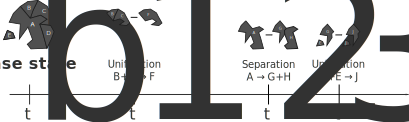
\includegraphics[width=0.8\textwidth]{graphics/basics/stdm/event-based_spatio-temporal_data_model}
%   \caption{The Event-Based Spatio-Temporal Data Model}
%   \label{fig:event-based_spatio-temporal_data_model}


A main problem is to maintain the integrity of the spatial topology when a new change gets inserted not at the end of the list. A simple example shows that problem: Given geo-object $X$ is part of the inital base configuration at change $t_b$. At a later change, e.g. $t_y$ $X$ gets replaced by object $Y$. If a new change that updates $X$ to $X'$ gets inserted before at time point $t_x < t_y$, then $t_y$ is not integer anymore, because object $X$ does not exist. That is why on insertion of a change, all succeeding changes have to be tested for integrity and it might be necessary to update later changes.


% subsection computational_model (end)

% section histoglobe_application (end)

% chapter development (end)

% ==============================================================================

\vspace{2em}
transition to next chapter